%% This document gives an example on how to use the ntnubachelorthesis
%% LaTeX document class.
%% Use oneside for PDF delivery and twoside for printing in a book style
%% use language english, norsk, nynorsk and one of the following shortenings
%%  ``BSP'' Bachelor i Spillprogrammering,\\
%%  ``BRD'' Bachelor i drift av nettverk og datasystemer,\\
%%  ``BIS'' Bachelor i Informasjonssikkerhet,\\
%%  ``BPU'' Bachelor i Programvareutvikling, \\
%%  ``BIND'' Bachelor i Ingeniorfad - data, \\
%%  ``BADR'' Bachelor i drift av datasystemer, \\
%%  ``BIT'' Bachelor i informatikk, \\
%%  ``BABED'' Bachelor i IT-støttet bedriftsutvikling.
%%   for example \documentclass[BIS,norsk,twoside]{ntnuthesis/ntnubachelorthesis}

\documentclass[BIS,norsk,oneside]{ntnuthesis/ntnubachelorthesis}
\thesistitle{Case 1: Ulovlig fildeling på skolenettet}
\thesisshorttitle{Case 1: Ulovlig fildeling på skolenettet}
\thesisauthor{Philip Nyblom, Fredrik Theien, Thomas Huse, Ole Martin Søgnen}
\thesisdate{16.05.2018}

\usepackage{csvsimple}
\usepackage{booktabs}
\usepackage{gnuplottex}
\usepackage[T1]{fontenc}
\usepackage[utf8]{inputenc}     % For utf8 encoded .tex files because...
\usepackage[norsk]{babel}       % For Norwegian labeling
\usepackage{graphicx}           % For inclusion of graphics
\PassOptionsToPackage{hyphens}{url}
\usepackage{url}
\usepackage{hyperref}    % For cross references in pdf
\usepackage{tabularx}
\usepackage[table]{xcolor}
\usepackage{placeins}
\usepackage{pdfpages}
\usepackage{enumitem}
\usepackage{multirow}
\usepackage{lscape}
\usepackage{bigstrut}
\usepackage{verbatim}
\usepackage{float}


\definecolor{darkgreen}{rgb}{0,0.5,0}
\definecolor{darkred}{rgb}{0.5,0.0,0}

\lstset{        basicstyle=\ttfamily,
                keywordstyle=\color{blue}\ttfamily,
                stringstyle=\color{darkred}\ttfamily,
                commentstyle=\color{darkgreen}\ttfamily,
}


%Typesetting of C++
\newcommand{\CPP}[0]{{C\nolinebreak[4]\hspace{-.1em}\raisebox{.1ex}{\small\bf +\hspace{-.1em}+\ }}}



%\newcommand{\comment}[1]{\textcolor{blue}{\emph{#1}}}  %% use of the colour and you can see how to use commands with parts \comment{so what}

%% The class files defines these two
%% \newcommand{\NTNU}{Norwegian University for Science and Technology} %

% you can create you one #define like structures using the \newcommand feature
% you can change behaviour using \renewcommand

\newcommand{\com}[1]{{\color{red}#1}} % supervisor comment
%\renewcommand{\com}[1]{} %remove starting % to remove supervisor comments
% This will appear in text \com{Lecuters comment} and be visible unless you uncomment
% the renewcommand line.

\newcommand{\todo}[1]{{\color{green}#1}} % items to do
%\renewcommand{\todo}[1]{} %remove starting % to remove items to do

\newcommand{\n}[1]{{\color{blue}#1}} % other comment
%\renewcommand{\n}[1]{} %remove starting % to remove notes

\newcommand{\dn}[1]{} % add the d to a note to say that you have finished with it.

\newcommand{\gj}{NTNU i Gj\o{}vik}


% Norwegian Characters,  needs the {} or to be separate from the next letters
% \o{}   \aa{}   \ae{}   so at the end of a word you can use \o  \aa   \ae
% \O{}   \AA{}   \AE{}   you can also just leave a space and latex will remove it
%    eg, NTNU i Gj\o vik  or NTNU i Gj\o{}vik

\graphicspath{ {bilder/} }

\begin{document}

\thesistitlepage

\tableofcontents
\listoffigures
\listoftables
\lstlistoflistings

\chapter*{Kortfattet sammendrag}
Kommer...
\chapter{Introduksjon}
Rotårsaksanalyser er et lite brukt verktøy innen informasjonssikkerhet, men er av økende betydning. Vanlig tilnærming til informasjonssikkerhetsstyring er å utføre en risiko-og sårbarhetsanalyse (ROS-analyse) for så å gjennomføre tiltak som fører risikoene til et akseptabelt nivå. En annen hyppig brukt tilnærming er hendelseshåndtering der en planlegger hvordan det skal responderes på hendelser etter de er inntruffet. Rotårsaksanalyse skiller seg fra disse ved å gå i dybden på problemet, kartlegge hva slags rotårsaker som står bak, og innføre tiltak for å fjerne disse helt.

\section{Oppgavebeskrivelse}
Denne rapporten er en delrapport i en større oppgave om rotårsaksanalyse. Dette caset går inn på rotårsaken til at brukere på skolenettet til NTNU laster ned opphavsrettsbeskyttet materiale. I denne rapporten bruker vi ordet fildeling når vi omtaler deling av filer gjennom torrents. Annen fildeling går ikke under vårt bruk av begrepet og heller ikke under problemstillingen vår. Vi bruker fortsatt begrepet Torrents når vi snakker om selve teknologien og sporingen av dem.

Hver måned får NTNU ca. 150 og 200 unike notifikasjoner om brudd på opphavsretten ved ulovlig fildeling. Vi kan se at dette nummeret går kraftig ned i sommermånedene, som kan tilsi at studentene er hovedgrunnen til bruddene på opphavsrett. Se figur \ref{fig:copyright} under for en grafisk illustrasjon av antall notifikasjoner for brudd på opphavsrett.

\begin{figure}[H]
    \centering
    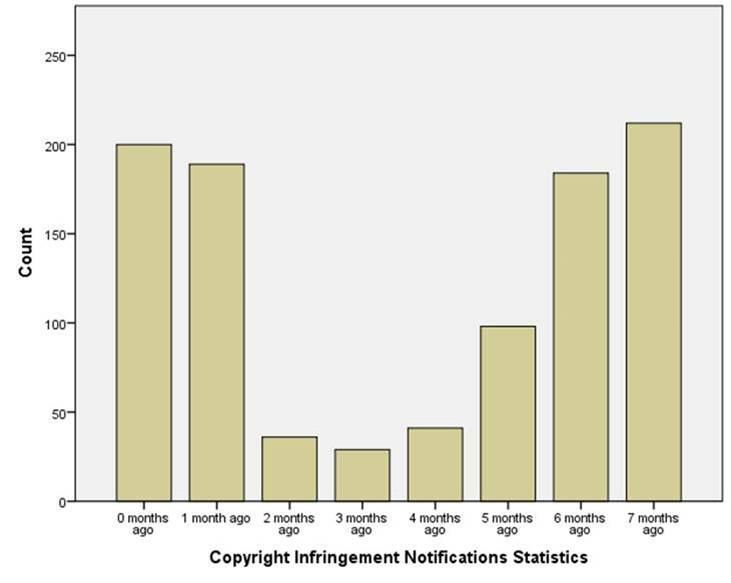
\includegraphics[scale=0.8]{copyright}
    \label{fig:copyright}
    \caption[Copyright Infringement Notifications]{Copyright Infringement Notifications}
\end{figure}

\begin{comment}
\begin{table} [h]
    \begin{tabular}{ | m{12em} | m{12em} | m{12em} | }
        \hline
            \cellcolor{yellow} & \cellcolor{yellow} Breaches & \cellcolor{yellow} Copyright breach/Piracy\\
        \hline
            Policy Violation & Information Security Policy & 2 \\
        \hline
             & IT Policy & 43 \\
        \hline
    \end{tabular}
    \caption{Oversikt over kvantiteten av brudd på policy}
    \label{kritisk_tabell_1}
\end{table}
\end{comment}

I denne oppgaven er vårt mål å finne rotårsakene til ulovlig fildeling og ikke å avdekke noen for det. Derfor er alle spørreundersøkelser anonyme. Dette presiseres også til intervjuobjektene under intervjuet.

\section{Metode}
Metodebruken i denne undersøkelsen er delt inn i syv steg som vist i figur \ref{fig:prosess} under. I hvert steg av denne prosessen brukes det ulike verktøy for å hjelpe til med å forstå problemet, finne rotårsak, og tilslutt implementere tiltak for å eliminere årsakene. 
\begin{figure}[H]
    \centering
    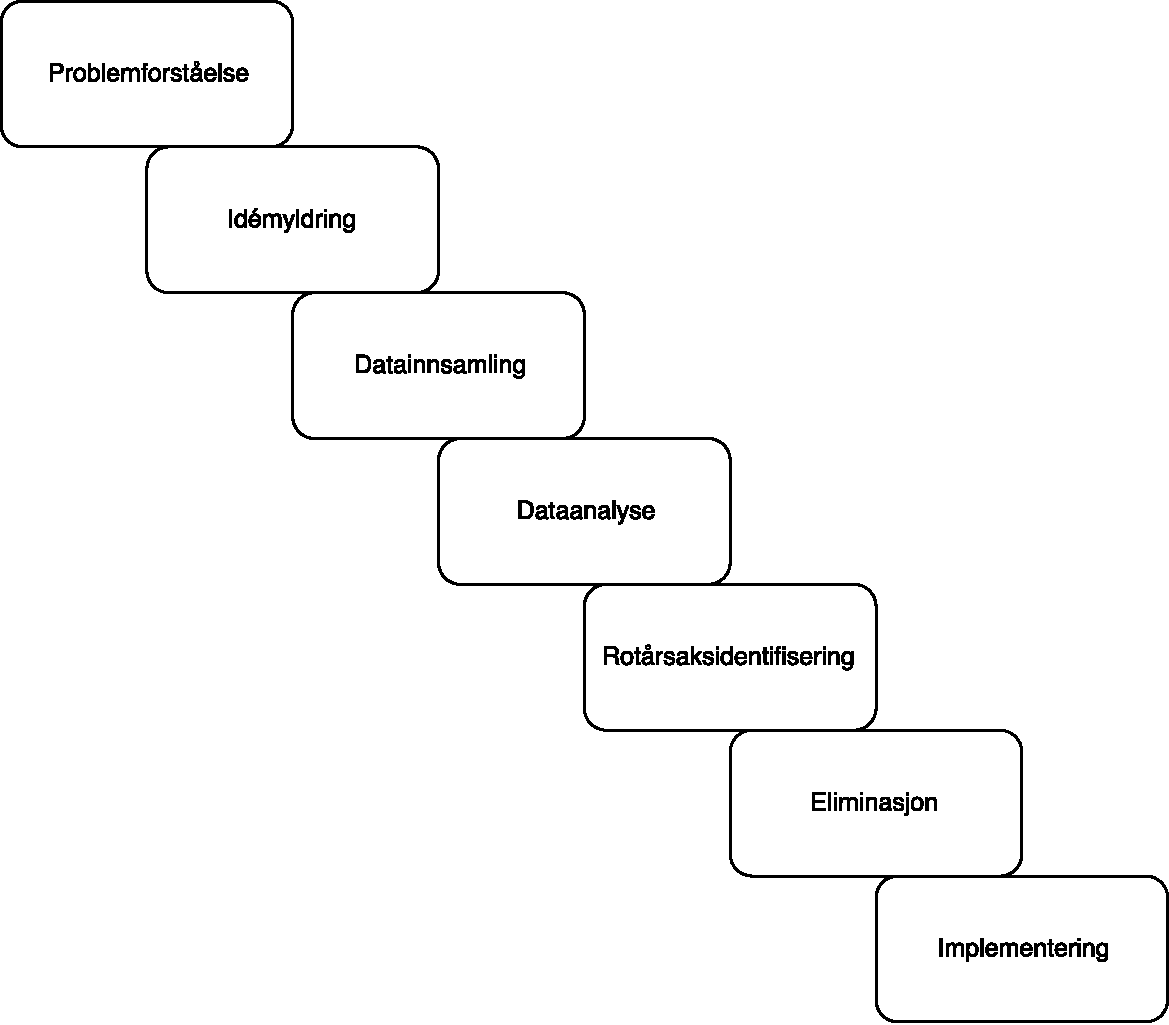
\includegraphics[scale=0.6]{prosess}
    \label{fig:prosess}
    \caption[Rotårsaksanalyseprosessen]{Rotårsaksanalyseprosessen definert av Andersen og Fagerli}
\end{figure}
\chapter{Problemforståelse}
Denne fasen eksisterer for å passe på at en har forstått problemet i dypere detalj. Verktøyene som er relevante å bruke skal gi en bedre forståelse av blant annet omfanget og de ulike aspektene ved et problem. Jo bedre tilgang en har på logger og dokumentasjon, jo bedre vil denne fasen kunne utføres. Siden vi har liten erfaring med bruk av verktøy vil vi prøve ut to i denne analysen. Kritiske hendelser for å undersøke hva som blir lastet ned, og flytdiagram for å kartlegge hendelsesforløpet til en som laster ned.

\section{Flytdiagram}
Et flytdiagram er et diagram som viser en flyt av aktiviteter i en prosess eller handling. Flytdiagrammer kan bli brukt til å kartlegge en prosess for å muligens illustrere hvor problemet ligger, eller for å skape en grunnleggende forståelse av prosessen som har innflytelse på problemet. 

\subsection{Ønsket utbytte}
Her prøver vi å kartlegge hendelsesforløpet, og hvordan bruksmønsteret til en bruker av nettet til NTNU kan se ut, da med fokus på fildeling. Vi håper at dette kan gi oss en mer helhetlig forståelse av hva som kan være årsaken til fildeling, og kanskje vi kan bruke dette til å komme opp med tiltak senere i prosessen.

\subsection{Gjennomføring}
Vi fulgte metoden for å lage et flytdiagram, fra boken om rotårsaksanalyse \cite{RCA}.
\begin{enumerate}
    \item Vi samlet alle på gruppen for å diskutere prosessen, og hadde med oss post-it lapper
    \item Vi definerte brukerne som studenter ved NTNU og da, antageligvis mest studenter som bor på studenthybler.
    \item Vi definerte hvilke aktiviteter som må bli gjort/være tilstede for at skolen skal få et notis.
    \item Så flyttet vi rundt på lappene til de kom i en naturlig rekkefølge.
\end{enumerate}


For å forstå problemet lagde vi et flytdiagram for å få en bedre forståelse av hendelsesforløpet når noen driver med fildeling.

\subsection{Resultater}
Flytdiagrammet som ble laget kan sees under. Først kobles en bruker seg til skolenettet, enten gjennom VPN eller direkte fra campus eller studenthybler. Deretter velger brukeren enten å bruke nettet vanlig eller starter å laste ned filer, hvis brukereren bruker det vanlig bryr vi oss ikke om disse. Når vedkommende som har bestemt seg for å laste ned skal laste ned har han muligheten til å gjøre dette gjennom en privat nedlastingsside. Vi gjør den antagelsen her at private tjenester ikke er med i statistikken fra skolen og at det ikke kommer noen opphavsrettsnotiser fra brukere som bruker private tjenester. Med private tjenester mener vi lukkede nettsamfunn som bare er til for å distribuere opphavsrettsbeskyttet materiale gratis. Det neste som kan skje med de som bruker offentlige tjenester er at de torrentene de laster ned blir sporet, og da får domeneeier et notis om ulovlig nedlasting.
\begin{figure}[H]
    \centering
    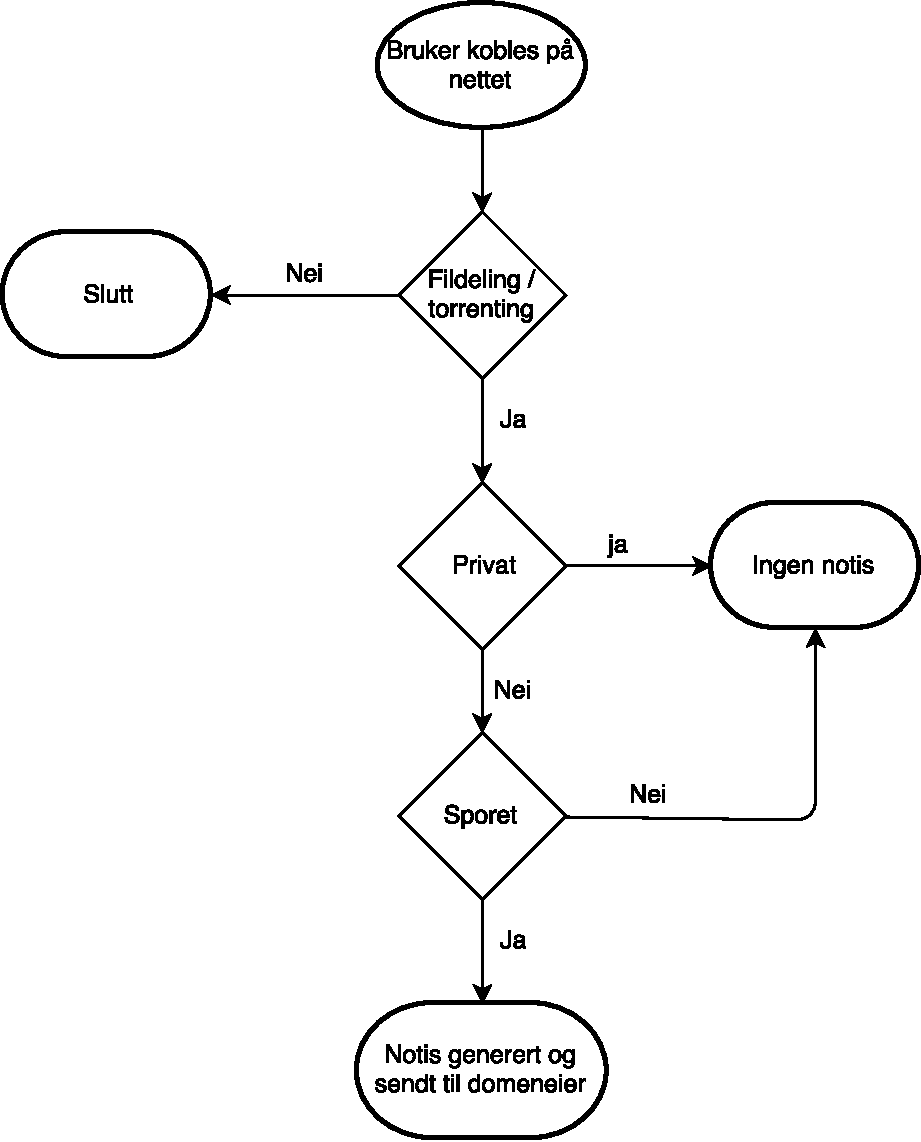
\includegraphics[scale=0.5]{case_1/bilder/Flowchart.pdf}
    \label{fig:Flytdiagram}
    \caption[Flytdiagram for fildeling]{Flytdiagram for fildeling}
\end{figure}

\subsection{Konklusjon av verktøyet}
Vi følte verktøyet fungerte godt for å få et overblikk på hvordan situasjonen med torrenting fungerte. Eneste negative med verktøyet er at det krever ganske god kjennskap til mulige hendelsesforløp, noe som kan være negativt om man ikke kjenner godt til problemet fra før. 

\section{Kritiske hendelser}
For å gå dypere i detalj har vi tatt en titt på kritiske hendelser som inngår i problemstillingen. Vi har valgt å dele opp problemet i mindre stykker for å spørre studenter som bor i SiT-bolig om hva de laster ned hvis de først gjør det. 

\subsection{Ønsket utbytte}
Ved bruk av dette verktøyet ønsker vi å få en dypere forståelse av hva studentene laster ned slik at vi kan se om det er noen kategorier som er mest fremtredende. Dette kan føre til at vi blir mer effektive i senere arbeid da vi kan fokusere på det som er viktigst.

\subsection{Gjennomføring}
Det første som ble gjort var å definere de mest relevante kategoriene av nedlastningsmateriale. Dette ble basert på egen erfaring med blant annet hyppigheten til de ulike kategoriene. Vi hadde en viss anelse om hvilke som var de store synderne, men ønsket å bekrefte våre mistanker. Følgende kategorier ble fremhevet: 
\begin{itemize}
    \item Filmer og serier
    \item Skolebøker
    \item Programvare til skolebruk
    \item Programvare og bøker utenom skolebruk
    \item Spill
    \item Musikk
    \item Annet
\end{itemize}

Deretter var det klart for utspørring. Dette var i stor grad uformelle ``intervjuer'' med få spørsmål. Det viktigste vi trengte å vite var om personen bodde i SiT-bolig, siden det er bare beboere derfra som er relevante i vår problemstilling, og fra hvilke kategorier de laster ned fra. Resultatene ble fortløpende ført inn i statistikken. De fleste som ble spurt studerte informatikk, men det ble også spurt noen fra andre linjer for å prøve å balansere det ut. Intervjuobjektene var i stor grad bekjente vi visste bodde i SIT Bolig, og derfor var det en overvekt av IT studenter.

Spørsmål stilt til intervjuobjekter:
\begin{itemize}
    \item Bor du, eller har du bodd i SiT-bolig i løpet av studiet? (Hvis nei, avslutt intervju)
    \item Bruker du, eller har du brukt Torrents til å laste ned opphavsrettsbeskyttet materiale mens du bodde i SiT-bolig? Hvis ja, hvilke av følgende kategorier laster du ned fra? (Viser kategoriene)
\end{itemize}

\noindent Dette er resultatet fra spørringene: \\
\indent Antall spurt: 13 \\
\indent Antall som aldri laster ned: 4
\begin{table} [H]
    \begin{tabular}{ | m{18em} | m{18em} | }
        \hline
            \cellcolor{yellow} Fildelingskategori & \cellcolor{yellow} Frekvens \\
        \hline
            Filmer og serier & 8  \\
        \hline
            Spill & 3 \\
        \hline
            Skolebøker & 2 \\
        \hline
            Musikk & 2 \\
        \hline
            Programvare og bøker utenom skolebruk & 1 \\
        \hline
            Programvare til skolebruk & 0 \\
        \hline
            Annet & 0 \\
        \hline
    \end{tabular}
    \caption{Oversikt over kvantiteten av kritiske hendelser ved torrenting av opphavsrettsbeskyttet materiale}
    \label{kritisk_tabell_1}
\end{table}

Merk: Hver person kan svare at de laster ned fra flere kategorier.

\noindent Vi kan se at det er filmer og serier som er den med størst frekvens i undersøkelsen, noe som bekreftet vår hypotese. Dette funnet vil tilsi at vi kan fokusere mye mer på filmer og serier senere i prosessen siden vi vet dette er en stor del av problemet. 

\subsection{Konklusjon av verktøyet}
Verktøyet bekreftet vår hypotese i at det meste som blir lastet ned på skolens nett er filmer og serier. Dette kan tas til videre betraktning senere i rotårsaksanalysen. Verktøyet fungerte bra og ga oss den informasjonen vi var ute etter. Den fungerer også greit om man ikke har en hypotese om omfang på forhånd slik vi hadde, så lenge en er flinke med idémyldring av mulige kategorier. 
\chapter{Idémyldring}
I dette steget i prosessen er målet å generere en liste over det vi tror kan være mulige årsaker til problemet. Det er en del forskjellige verktøy en kan bruke for å oppnå dette, men vi har valgt å benytte Idémyldring på bakgrunn av verktøyets egenskap til å generere mange idéer hurtig.

\section{Idémyldring}
I rotårsaksanalyse finnes det to ulike måter å gjennomføre Idémyldring på, Strukturert- og Ustrukturert Idémyldring. I den strukturerte versjonen får hver deltaker sin tur til å komme med en idé, og dette sikrer at alle får delta like mye. På den ustrukturerte måten kan alle komme med idéer når de dukker opp, og fungerer mye mer spontant enn den strukturelle. Det er spesielt viktig å ikke omformulere eller diskutere forslagene etterhvert som de kommer, dette skal gjøres etter Idémyldringsøkten er over.

\subsection{Ønsket utbytte}
Ønsket utbytte i denne delen er en mengde idéer som kan legges til grunn når det utføres statistisk arbeid på rotårsakene. Det er spesielt ønskelig å kunne ende opp å utvikle spørsmål til brukerundersøkelser basert på noen av disse årsakene.

\subsection{Gjennomførelse}
Det første som ble gjort når økten startet var å kommunisere og skrive opp problemstillingen på en tavle. Vi valgte å strukturere Idémyldringen som et tankekart ettersom dette var en kjent løsning for gruppen, og brukte den ustrukturerte tilnærmingen til Idémyldringen på grunn av dens uformelle og spontane natur. 

Det første problemet vi så på var hvorfor personer bruker Torrents til å laste ned opphavsrettsbeskyttet materiale. Når idéstrømmen begynte å gå langsomt, stoppet vi og vurderte det vi hadde kommet fram til. Vi kom blant annet fram til at vi burde spesifisere problemstillingen ytterligere og valgte derfor å spesifisere den til hvorfor folk laster ned på skolenettet. Vi forkortet dette til: ``Hvorfor Torrenting på skolenettet'' for enkelthets skyld. Det ble kjørt enda en økt med denne nye problemstillingen og fikk mer spesifikke resultater. 

\subsection{Resultater}
Etter øktene var ferdig ble det gjort en vurdering av resultatene og de ble kategorisert i henhold til likhetstrekk, under en fellesnevner som for eksempel Økonomi. Resultater og gruppering er som vist i figur \ref{fig:idemyldring} under.

\begin{figure}[H]
    \centering    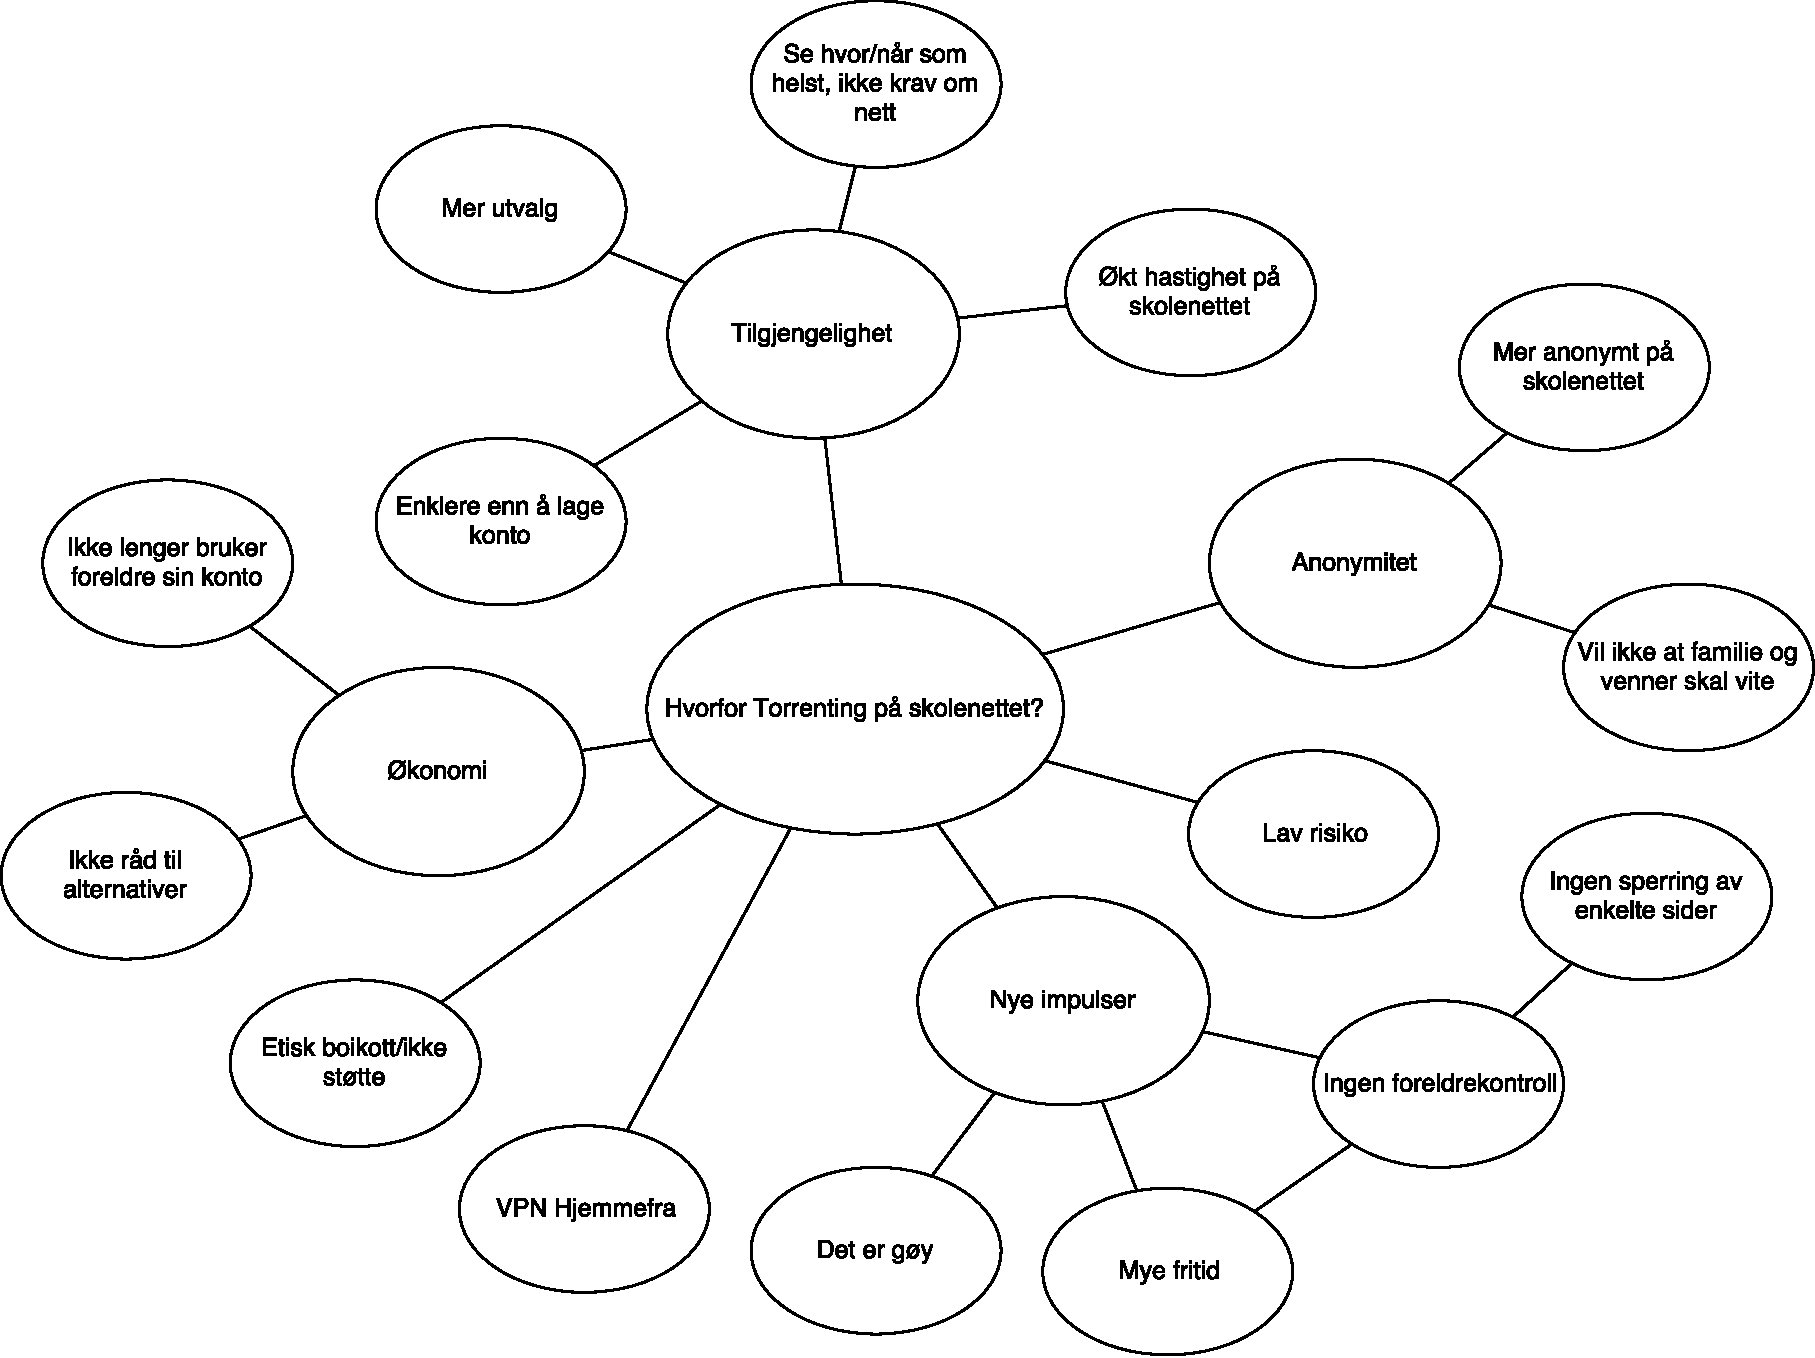
\includegraphics[scale=0.45]{case_1/bilder/idemyldring}
    \caption[Idémyldring]{Resultater og gruppering av idémyldringen}
    \label{fig:idemyldring}
\end{figure}

Resultatene er gruppert inn i fire hovedkategorier, Økonomi (som går på kjøpekraften til den enkelte person), Tilgjengelighet (hvor god tilgang en har på tjenester), Anonymitet (foreldre kunne blant annet overvåke før, samt føler seg tryggere når det er flere på samme nett) og Nye impulser (mer frihet og fritid, og påvirkning av nedlastningskulturen).

Merk at noen årsaker kunne ikke plasseres i én kategori og er derfor direkte knyttet til problemstillingen. 


\subsection{Konklusjon av verktøyet}
Dette var en effektiv metode for å få en overordnet oversikt av hva årsakene kan være til at noen velger å laste ned opphavsrettsbeskyttet materiale, spesielt på skolenettet. Verktøyet fungerte bra i denne sammenhengen fordi gruppen hadde en del basiskunnskap om temaet fra før. Vi antar at en slik metode vil fungere dårligere dersom problemet ikke er forstått godt nok og/eller det er lite kunnskap om problemstillingen på forhånd.
\chapter{Datainnsamling}
Datainnsamlingen er kritisk til resultatet av oppgaven. Målet i denne fasen er å samle inn et så bredt aspekt av informasjon som mulig gjennom et par mulige verktøy og teknikker beskrevet i boka om rotårsaksanalyse\cite{RCA}. Vi har valgt å bruke spørreundersøkelser som et verktøy for å hente inn informasjon om dette caset fordi vi skal hente inn informasjon fra et stort antall studenter som bor i studentbyene SiT administrerer.

\section{Elektronisk spørreundersøkelse}
Det finnes i hovedsak to forskjellige undersøkelsestyper, kvantitative og kvalitative spørreundersøkelser. Kvalitative undersøkelser går ut på å spørre utvalgte personer, og er ofte mye mer detaljerte og samler svar av høyere kvalitet. Kvantitative undersøkelser fungerer motsatt i at det er fokus på mange tilbakemeldinger slik at en kan senke usikkerhet knyttet til svarkvalitet. \cite{} I vår situasjon har vi valgt kvantitativ undersøkelse på bakgrunn av et par faktorer. For det første ønsker vi at undersøkelsen skal være helt anonym, siden spørsmålene omhandler potensielle lovbrudd. For det andre er målgruppen et stort antall personer, så det kan være nyttig å samle inn data fra så mange av de som mulig.

\subsection{Ønsket utbytte}
Det vi ønsker å få ut av spørreundersøkelsen er data på utvalgte spørsmål vi mener er relevante for oppgaven. Denne fasen er utelukkende for å innhente informasjon, bearbeiding av informasjonen skjer i neste fase. Spørsmålene er utarbeidet for å utforske hvorfor studenter som bor i studentbyer laster ned opphavsrettsbeskyttet materiale, som blant annet inkluderer undersøkelse av økonomiske perspektiver og tilgjengelighet på tjenester. I tillegg ønsker vi også innsikt i hvordan dette kan stoppes. 

Hypotesen vi går inn i undersøkelsen med er at folk laster ned opphavsrettsbeskyttet materiale fordi det er lett tilgjengelig, tilknyttet liten til ingen kostnad og ikke minst fordi det er svært lav risiko for represalier.

\subsection{Gjennomførelse}
Prosessen startet ved å utforme spørreundersøkelsen. En god undersøkelse vil alltid kreve kartlegging av demografi, og i vår undersøkelse valgte vi å kartlegge studentby, kjønn, alder og fakultet. Kjønn og alder er ganske selvforklarende, mens studentby ble valgt på bakgrunn av at Kallerud har mye raskere nedlasting- og opplastingshastighet enn de andre stedene. Vi anså også at det ville være forskjell på hvor mange som laster ned mellom for eksempel informatikkstudiene og helsestudiene. Videre ble resultatene i de foregående fasene brukt til å utforme spørsmålene. Spørreundersøkelsen inkluderer spørsmål om hvor godt en rekke påstander stemmer for den enkelte der respondentene svarer på en likert-skala fra 1-5, der 1 er i liten grad og 5 er i stor grad. Til slutt inkluderes det et spesielt viktig spørsmål om hva som skal til for at personen stopper med ulovlig nedlasting. Dette er et frisvar der vi kommer til å analysere individuelle svar hver for seg. Spørreundersøkelsen kan leses i sin helhet i \hyperref[undersokelse]{Vedlegg A}.
\newline
Det er alltid en stor utfordring å finne nok respondenter til spørreundersøkelser, og vi setter en del krav til antall respondenter og utfører en rekke tiltak for å oppnå nok besvarelser, slik at undersøkelsen kan si noe om rotårsaken med relativt høy sikkerhet. Det er et krav å få minst 30 besvarelser som hadde lastet ned opphavsrettsbeskyttet materiale mens de har bodd i hybelen. Videre er det også ønskelig med relativ likhet i antall respondenter mellom de ulike fakultetene og studentbyene. Det hadde vært ideelt med minst 30 respondenter i hver kategori her også, men det er ønsketenkning i denne sammenhengen. Under prosessen ble også totalt antall beboere fra alle studentbyene i SiT bolig kartlagt. Boligtorget ga oss innbyggertallene fra hver studentby, og vi regnet oss frem til totalt 522 beboere. Det er viktig å presisere at det kan være usikkerheter knyttet til disse tallene, siden det kan hende ikke alle boligene har en beboer.

Siden spørreundersøkelsen er elektronisk var et av de første tiltakene som ble gjennomført å spre den på relevante facebook-sider. Et av prosjektgruppens medlemmer jobber på Studenthuset her på Gjøvik, og fikk spørreundersøkelsen delt på deres facebook-side. Senere i prosessen ble også undersøkelsen delt på facebook-siden til linjeforeningen INGa og klassesidene til sykepleierne og webutvikling. Undersøkelsen ble også delt gjennom venner og bekjente; disse var for det meste informatikkstudenter. I tillegg ble det laget en plakat som ble hengt opp på oppslagstavler på skolen og i vaskeriene i de ulike studentbyene, og mange ble også plassert i postkassene til SiT boliger. Plakaten finnes i \hyperref[plakat]{Vedlegg B}. 

\subsection{Resultater}
Undersøkelsen endte med 97 svar totalt, dette er 18.6\% av de 522 beboerne i SiT bolig. Av disse var det 34 som svarte at de hadde lastet ned opphavsrettsbeskyttet materiale i hybelen, det er 35\% av de spurte. Videre resultater og analyse av disse blir diskutert i neste fase. 

\subsection{Konklusjon av verktøy}
Konklusjonen er at spørreundersøkelser er en effektiv metode for å samle inn store mengder data. En må likevel være konsekvent på tiltakene som iverksettes for å få inn respondenter. Det er også viktig i kvantitative spørreundersøkelser å få relativ likhet i demografien for å kunne si noe om de ulike kategoriene. Dette kan i noen tilfeller være krevende. En annen ting som er svært sentralt i bruk av verktøyet er utformingen av spørsmålene. Det er vanskelig å legge til spørsmål etter spørreundersøkelsen allerede er utsendt, og hva en da trenger ekstra informasjon må dette supplementeres i en mulig kvalitativ undersøkelse eller liknende. 
\chapter{Dataanalyse}
Denne fasen, og den foregående, er de vi har fokusert mest på i prosessen. Hvis en av de gjøres ufullstendig vil det være kritisk for resultatet av oppgaven. I denne fasen analyseres dataene som er samlet inn, og ved hjelp av statistiske verktøy kan vi trekke konklusjoner basert på svarene. Under dataanalysen kommer vi til å bruke generelle statistiske verktøy for å illustrere svarene og sammenhengene mellom de. Hovedfokuset i denne fasen er likevel å fokusere på de verktøyene som er beskrevet i boken om rotårsaksanalyse \cite{RCA}, men vi utelukker ikke bruk av annet vi anser som nyttig. Etter denne fasen ønsker vi å sitte igjen med mulige årsaker til at folk driver med ulovlig fildeling, samt andre relevante data relatert til fildeling. Verktøyet vi har brukt til å gjøre mesteparten av analysene er SPSS, et statistisk verktøy for å blant annet gjøre grafiske- og matematiske beregninger.

\section{Demografi}
I spørreundersøkelsen ble informasjon om fire forskjellige demografier samlet inn: Kjønn, fakultet, studentby og alder. Det er viktig å nevnte at det ikke ble samlet inn lik mengde svar fra alle kategoriene, så dette må vi tenke på når vi analyserer dataene. Det var for eksempel overvekt av menn som besvarte undersøkelsen. Av respondentene var det 27.8\% kvinner og 72.2\%. Det var også overvekt av personer som er mellom 20 og 25 år, disse tilsvarte 74.2\% av de spurte. På fakultet og studentby ønsket vi i hovedsak å få inn relativt spredte svar, men det ble overvekt av personer fra fakultet for informasjonsteknologi og elektroteknikk, og også en overvekt av personer fra Kallerud studentby. Disse inkluderte henholdsvis 50.5\% og 52\% av respondentene. De komplette frekvenstabellene over demografien finnes i \hyperref[frekvens]{Vedlegg C}.

\section{Analyse ved hjelp av histogram}
Histogrammer brukes til å vise distribusjonen og variasjonen i et spesifikt datasett. Hovedgrunnen til å bruke histogrammer er for å skape en visuell forståelse av dataene som en ellers ikke får fra tabeller o.l. Da blir det enklere å se korrelasjoner og sammenhenger i datasettet. Innen rotårsaksanalyse brukes det ofte for å visualisere hvilke mulige rotårsaker som er mest utbredt, og forstå distribusjonen av hendelser, problemer, årsaker, konsekvenser osv. \cite{RCA}

\subsection{Ønsket utbytte}
Ønsket utbytte ved bruk av histogrammer er en visualisering av de mest utbredte mulige rotårsakene, samt info om andre relevante aspekter ved oppgaven. Analyse av spørsmålene tilknyttet likert-skala er viktig for å finne mulige rotårsaker. Ellers ønsker vi også å finne sammenhenger mellom de ulike spørsmålene, for å se relevante korrelasjoner mellom de.


\subsection{Gjennomføring og resultater}
Vi starten analysen ved å undersøke hvor mange som faktisk laster ned av de spurte. Dette ble gjort i SPSS og arrangert etter prosentandel. Resultatet konkluderte med at det er 35\% som har lastet ned og 65\% som ikke har gjort det, som vist i histogrammet under.

\begin{figure}[H]
    \centering
    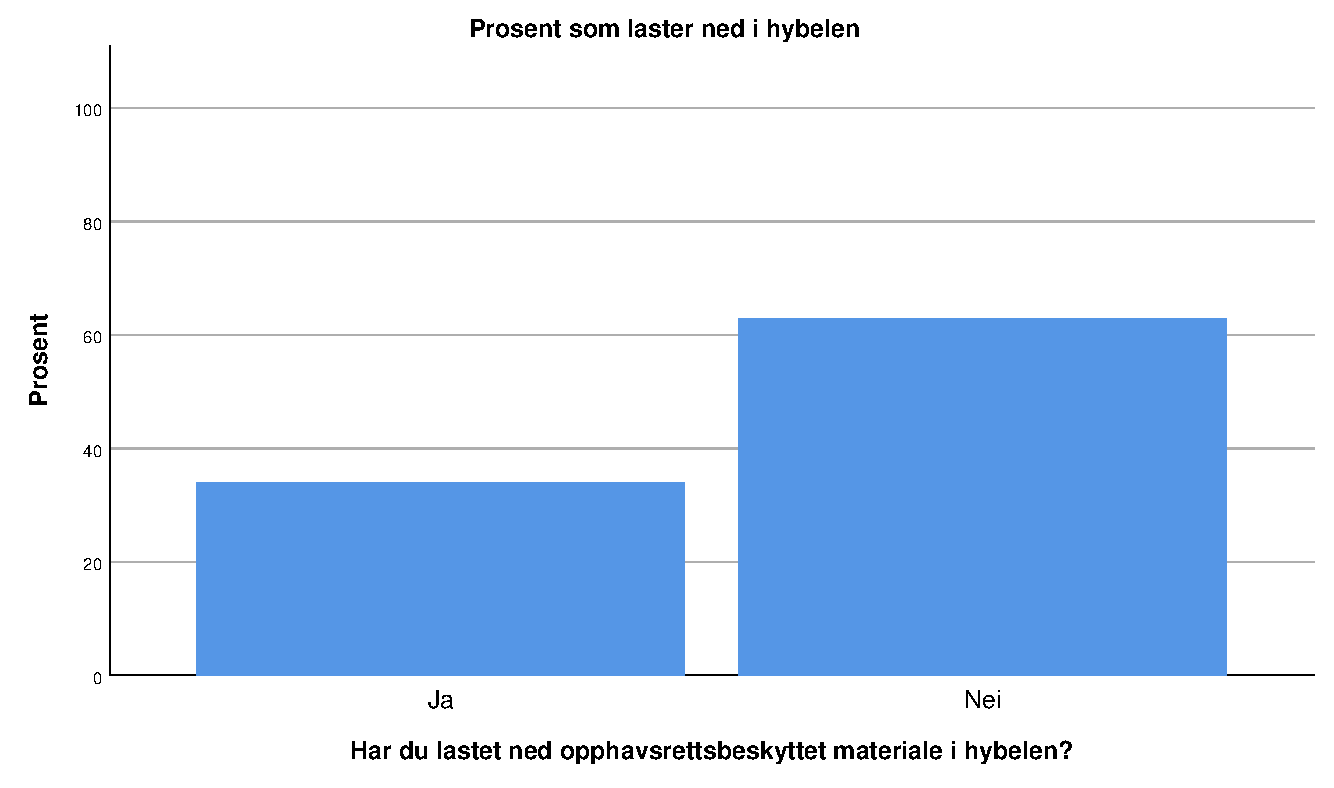
\includegraphics[scale=0.45]{case_1/bilder/lasterned.pdf}
    \label{fig:lasterned}
    \caption[Laster ned]{Hvor mange som laster ned av de spurte}
\end{figure}

Vi kan se på histogrammet at flertallet ikke laster ned, som var noe flere enn vi forventet, men det er fortsatt en stor andel som faktisk laster ned ulovlig. Det har også en liten innvirkning at en stor andel av respondentene kom fra informatikk- og datarelaterte studier, så vi kan fastslå at gjennomsnittet egentlig ligger noe lavere på nedlasting, men ikke med mye. Dette vises i \hyperref[fig:IT-lasterned]{følgende histogram}.

\subsubsection{Kjønnsforskjeller}
Vi ønsket også å undersøke om det er noen forskjeller i hvem som laster ned basert på kjønn. Under ser vi forholdet mellom kjønnene.
\begin{figure}[H]
    \centering
    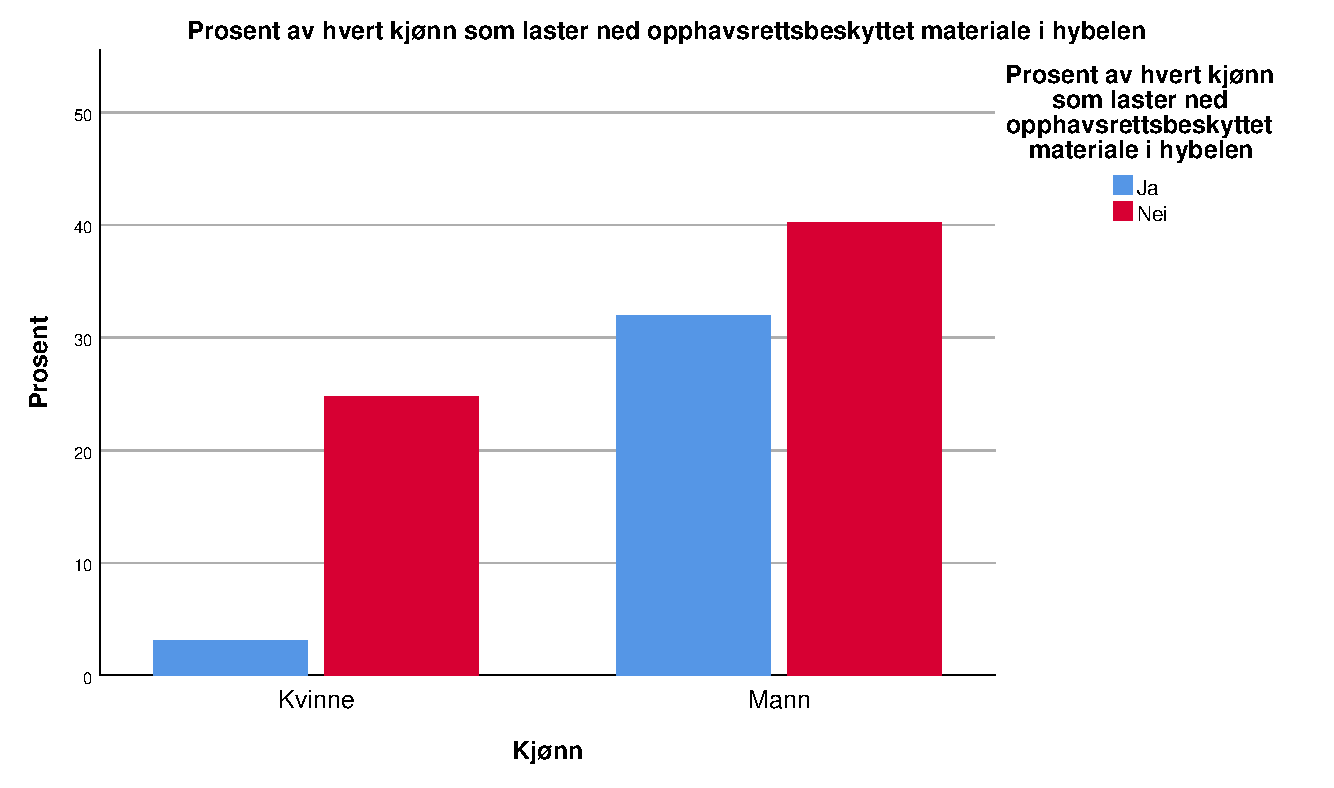
\includegraphics[scale=0.45]{case_1/bilder/kjonn_lasterned.pdf}
    \label{fig:kjønn_lasterned}
    \caption[Kjønn laster ned]{Hvor mange fra hvert kjønn som laster ned}
\end{figure}
Vi kan se over at det er i hovedsak menn som laster ned ulovlig, mens kvinner har svart at de i stor grad ikke laster ned. Dette blir selvfølgelig påvirket at det er få kvinner i IT-relaterte studier, som vi har funnet ut at utgjør noe mer av nedlastingen. Det er derimot vanskelig å vite helt sikkert om det er fordi kvinner er underrepresentert i IT studier som gir utslag, eller om det er kvinner generelt sett som ikke laster ned. Der er likevel en mer signifikant forskjell mellom kjønnene enn det er mellom IT studier og andre studier som vist i figur \ref{fig:IT-lasterned}, så vi velger å tolke det som at kvinner laster ned mindre enn menn.

\subsubsection{Forskjeller mellom studentbyer}
Samtlige studentbyer har et kablet nettverk av Uninett godt egnet for nedlasting, enten det er lovlig eller ulovlig nedlasting. Det er derimot noen forskjeller i hastighet på enkelte studentbyer. Nordbyen, Sørbyen og Sentrum har muligheten til 100Mbps nedlasting og 100Mbps opplasting, mens Kallerud har en øvre grense på hele 1000Mbps nedlasting og 1000Mbps opplasting. Dette er ti ganger hastigheten til de andre studentbyene. Derfor ønsket vi å undersøke om dette hadde noe relevans i forhold til hvor mange som laster ned ulovlig. 

\begin{figure}[H]
    \centering
    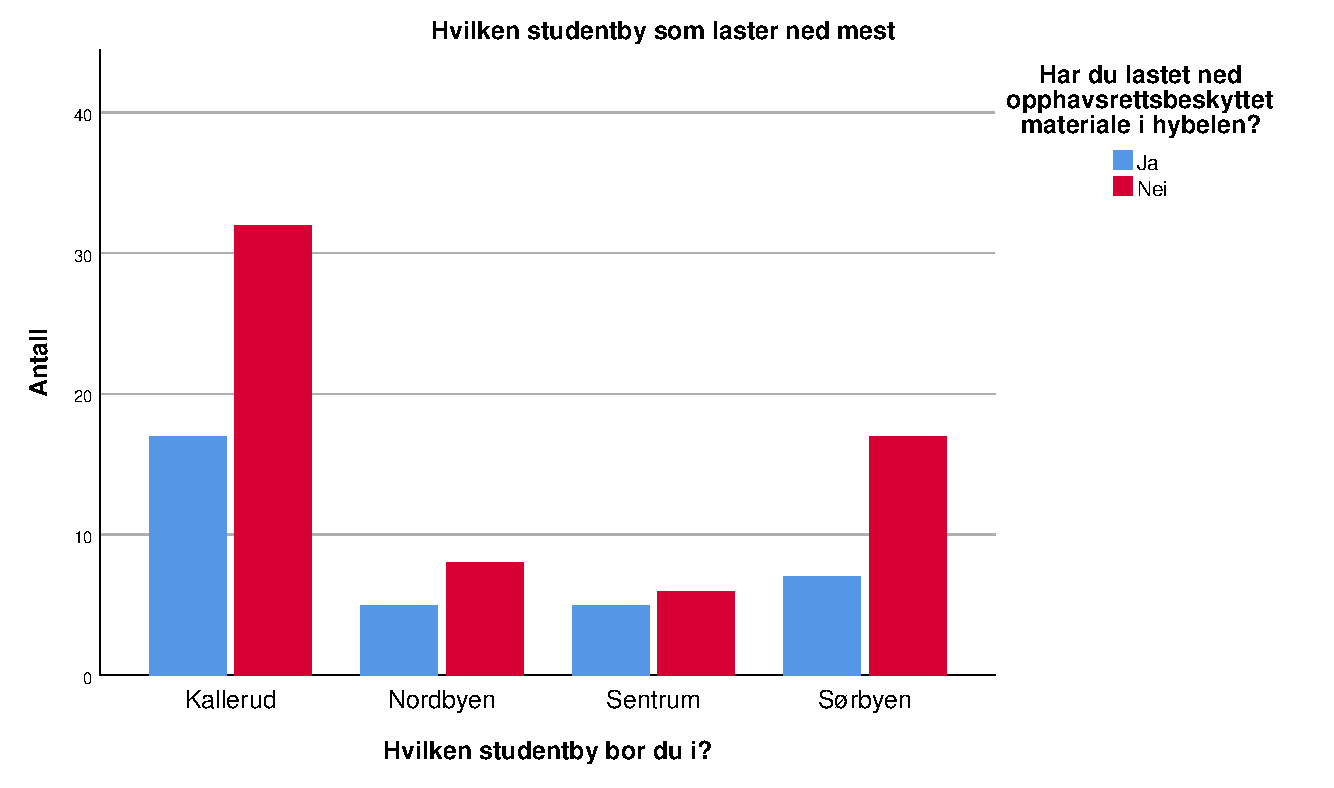
\includegraphics[scale=0.45]{case_1/bilder/studentby_lasterned.pdf}
    \label{fig:studentby_lasterned}
    \caption[Studentby laster ned]{Hvor mange fra hver studentby som laster ned}
\end{figure}

På grunn av lav oppslutning på Nordbyen og Sentrum er det vanskelig å si noe sikkert på dem, mens Kallerud og Sørbyen ikke varierer så veldig fra hverandre. Når vi bruker histogrammer ser vi ingen signifikant forskjell mellom studentbyene når det kommer til nedlasting som vi kan si med sikkerhet.

\subsubsection{Konsekvenser ved nedlasting}
Et spørsmål som ble spurt i spørreundersøkelsen var hvor godt kjent de var med mulige konsekvenser ved ulovlig nedlasting, og med det brudd på opphavsretten. Det kunne være relevant å se om det var noen spesiell sammenheng mellom de som ikke kjente til konsekvensene og de som lastet ned. 

\begin{figure}[H]
    \centering
    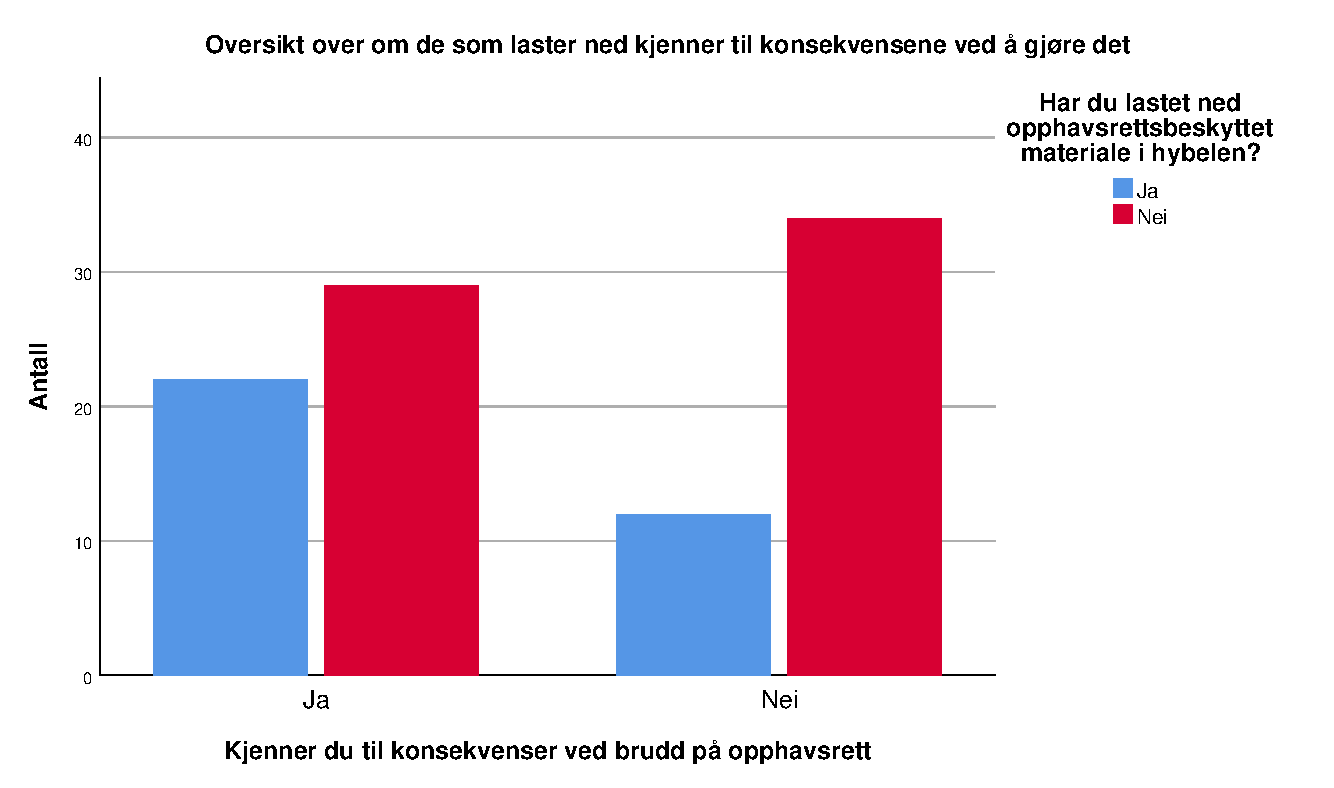
\includegraphics[scale=0.45]{case_1/bilder/konsekvens_lasterned.pdf}
    \label{fig:konsekvens_lasterned}
    \caption[Konsekvens av å laste ned]{Hvor mange som kjenner til konsekvenser ved å laste ned}
\end{figure}

Det viser seg faktisk at de som laster ned har en bedre kjennskap til konsekvensene enn de som ikke gjør det. Det kan kanskje ha noe å gjøre med at de er mer opptatt av problemområdet enn de som ikke laster ned. De som ikke laster ned i første omgang har kanskje ingen grunn til å sjekke konsekvensene av det. I tillegg fant vi ut at IT-studenter kjenner konsekvenser bedre enn de andre, og de har også høyere andel nedlastere. Vi prøvde å kjøre samme test på hvor godt de kjenner til IT-reglementet til NTNU \cite{ITReg} og kom til samme konklusjon som over. Dette histogrammet kan sees \hyperref[fig:reglement-lasterned]{her}. En grunn til dette er også igjen at IT-studenter kjenner bedre til IT reglementet, som vist \hyperref[fig:reglement-fakultet]{her}, og de er i overvekt. Så dette må tas i betraktning. 

En mulig teori vi ønsket å prøve ut var om mange som lastet ned ikke kjente til konsekvensene ved ulovlig nedlasting eller NTNU sitt IT-reglementet, og lastet ned på grunn av det. Dette ble altså delvis motbevist.

\subsubsection{Årsaker til nedlasting}
I spørreundersøkelsen kom vi med seks påstander til hvorfor respondentene laster ned, som de besvarte på en likert-skala fra 1 til 5, der 1 er i liten grad og 5 er i stor grad. Etter å ha analysert alle seks påstandene ved hjelp av SPSS og histogrammer fant vi én påstand som hadde en graftopp der respondentene svarte positivt. De aller fleste svarte de var enige i at de lastet ned på grunn av tilgjengelighet.

\begin{figure}[H]
    \centering
    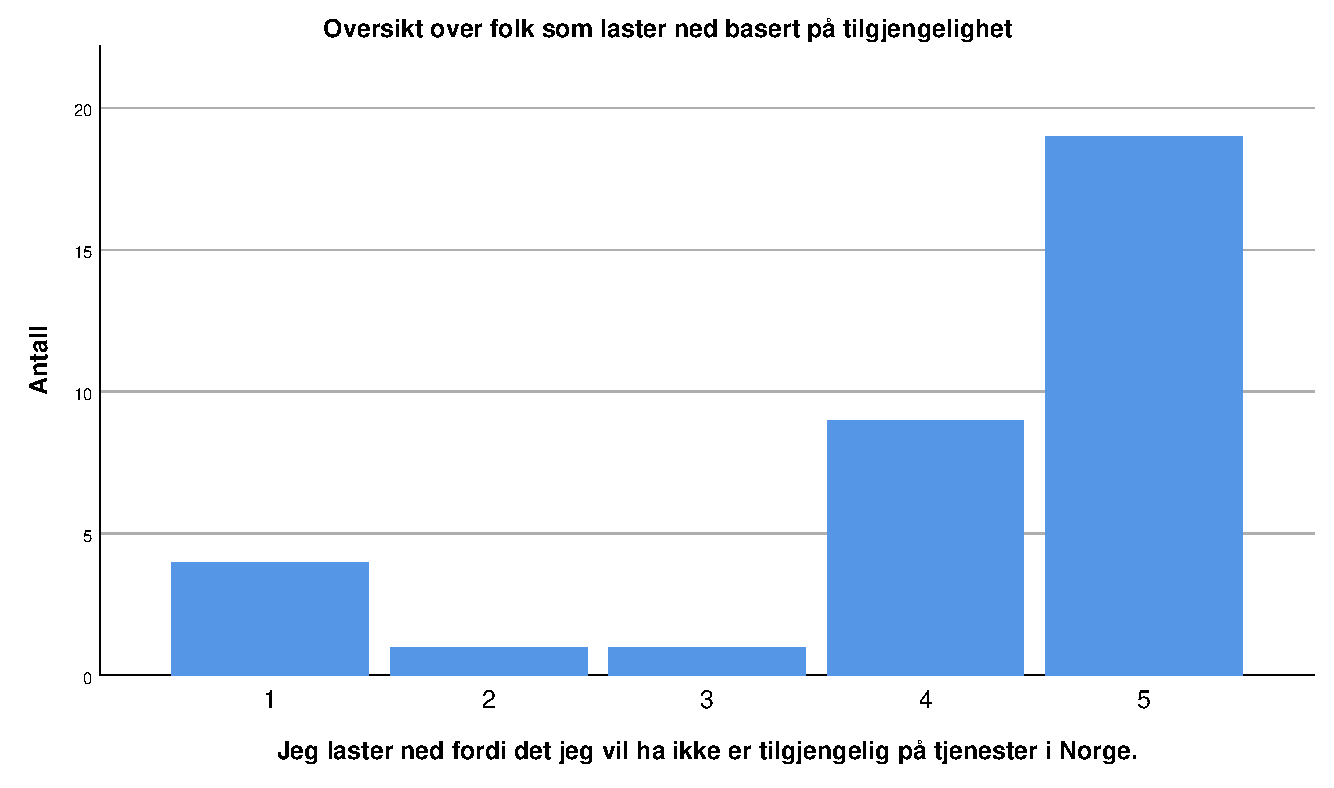
\includegraphics[scale=0.45]{case_1/bilder/tilgjengelighet.pdf}
    \label{fig:tilgjengelighet}
    \caption[Tilgjengelighet]{Hvor mange som laster ned av de spurte}
\end{figure}

Dette vil si at det er godt mulig at tilgjengeligheten er en årsak til om en laster ned eller ikke, og er verdt å dokumentere til videre analyse. Siden tilgjengelighet betyr så mye, var det naturlig å utforske det ytterligere. Vi fant ut at det kunne være relevant å vite om de som brydde seg om tilgjengelighet hadde tilgang på strømmetjenester, og i så fall hvor mange.

\begin{figure}[H]
    \centering
    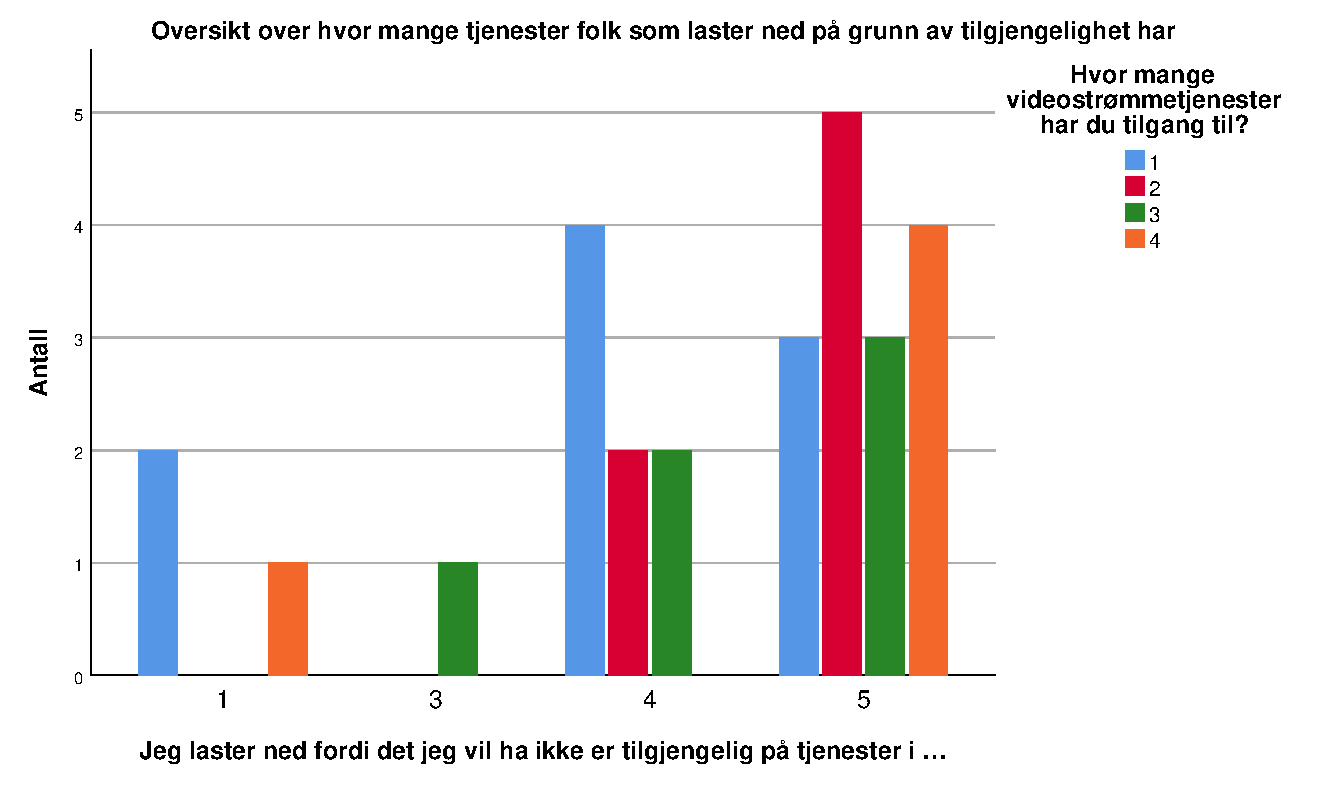
\includegraphics[scale=0.45]{case_1/bilder/tilgjengelighet_antallstromming.pdf}
    \label{fig:tilgjengelighet_antallstromming}
    \caption[Tilgjengelighet vs antall strømmetjenester]{Korrelasjonen mellom de som laster ned på grunn av tilgjengelighet og hvor mange tjenester de har tilgang på}
\end{figure}

Her viser det seg at de som laster ned på grunn av tilgjengelighet også har en god del strømmetjenester. Dette sier at mange av disse er storforbrukere av film og serier, og at det ikke har så mye å si om de har tilgang til tjenestene eller ikke. Dette vil muligens utelukke en løsning i form av at NTNU tilbyr en tjeneste siden de kommer til å laste ned uansett.

\subsection{Konklusjon av verktøy}
Histogrammer er et velkjent og godt verktøy innen statistikk og fungerer godt i mange forskjellige felt, inkludert rotårsaksanalyse.  Det fungerte også veldig bra i denne sammenhengen for å visualisere problemer knyttet til informasjonssikkerhet, og lettere forstå dataene. Siden dataene ble lettere å forstå førte det også til at vi hadde mulighet til å lage flere histogrammer for å analysere mange aspekter ved spørreundersøkelsen. Det negative med histogrammer er hvis de ulike dataene har stor forskjell på antall respondenter i de ulike kategoriene. Da kan det være vanskelig å se sammenhenger og korrelasjoner visuelt sett. Dette kan løses ved å ta et tilfeldig utvalg fra hver kategori og gruppere det opp mot det spørsmålet man ønsker å analysere det med. Da vil det være lettere å se korrelasjoner, men siden vi hadde for lite utvalg kunne vi ikke gjøre dette på alle dataene vi ønsket. Det er likevel enkelt å se korrelasjoner dersom det er signifikante forskjeller eller likheter.

%------------------------------------------------------ANOVA_ANALYSE----------------------------------------------------
\section{Statistisk analyse}
I denne delen benytter vi et par statistiske verktøy for å analysere dataene. Verktøyene vi har brukt er en independent-samples t-test og en one-way ANOVA. Begge disse ble beregnet i det statistiske verktøyet SPSS.


\subsection{Ønsket utbytte}
Vi ønsket å benytte en independent t-test for å undersøke forskjeller mellom variabler der den uavhengige variabelen bestod av to grupper. Vi ville utforske om det var noen signifikant forskjell når det kom til om folk laster ned, mellom Kallerud og de andre studentbyene. I tillegg ville vi se på om det var noen signifikante forskjeller mellom IT fakultetet og de andre fakultetene. Ønsket utbytte ved bruk av ANOVA-analysen er å gi oss et bilde av om påstandene har noen signifikant verdi knyttet til demografien.


\subsection{Independent-samples t-test}
Vi valgte å kjøre en independent-samples t-test for å undersøke om det at Kallerud har ti ganger så raskt nett har noen innvirkning på om en laster ned eller ikke. Vi delte opp Kallerud og de andre studentbyene hver for seg, og oversatte nei og ja svarene fra om du hadde lastet ned til henholdsvis 1 og 2. Under ser vi litt statistikk for svarene. 
\begin{figure}[H]
    \centering
    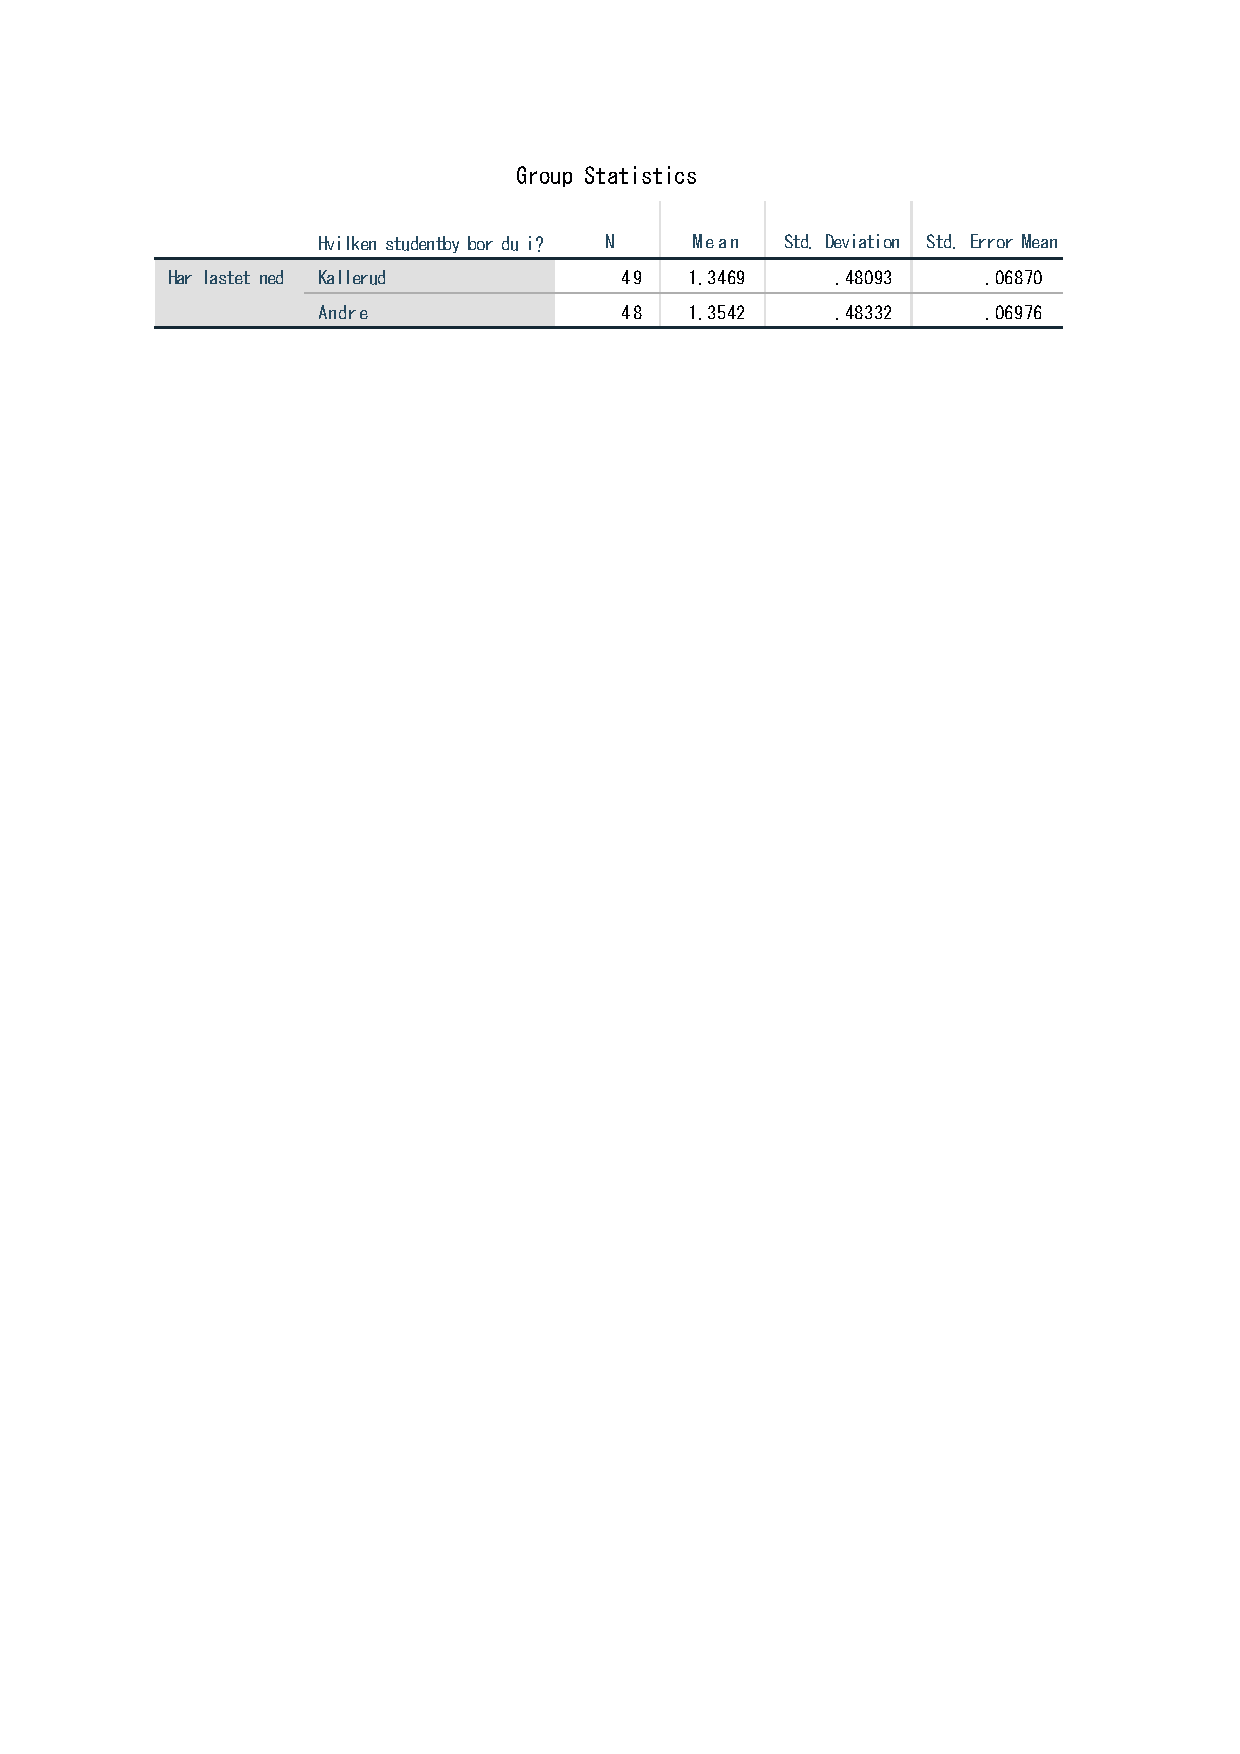
\includegraphics[scale=0.7]{case_1/bilder/studentby_lasterned_ttest_stats.pdf}
    \caption{Gruppestatistikk av studentbyer for om de laster ned eller ikke}
    \label{fig:studby_lasterned_ttest_stats}
\end{figure}

Vi kan allerede her se at svarene ikke differensierer noe særlig. I testen under ser vi selfølgelig derfor at det ikke er noen signifikans.

\begin{figure}[H]
    \centering
    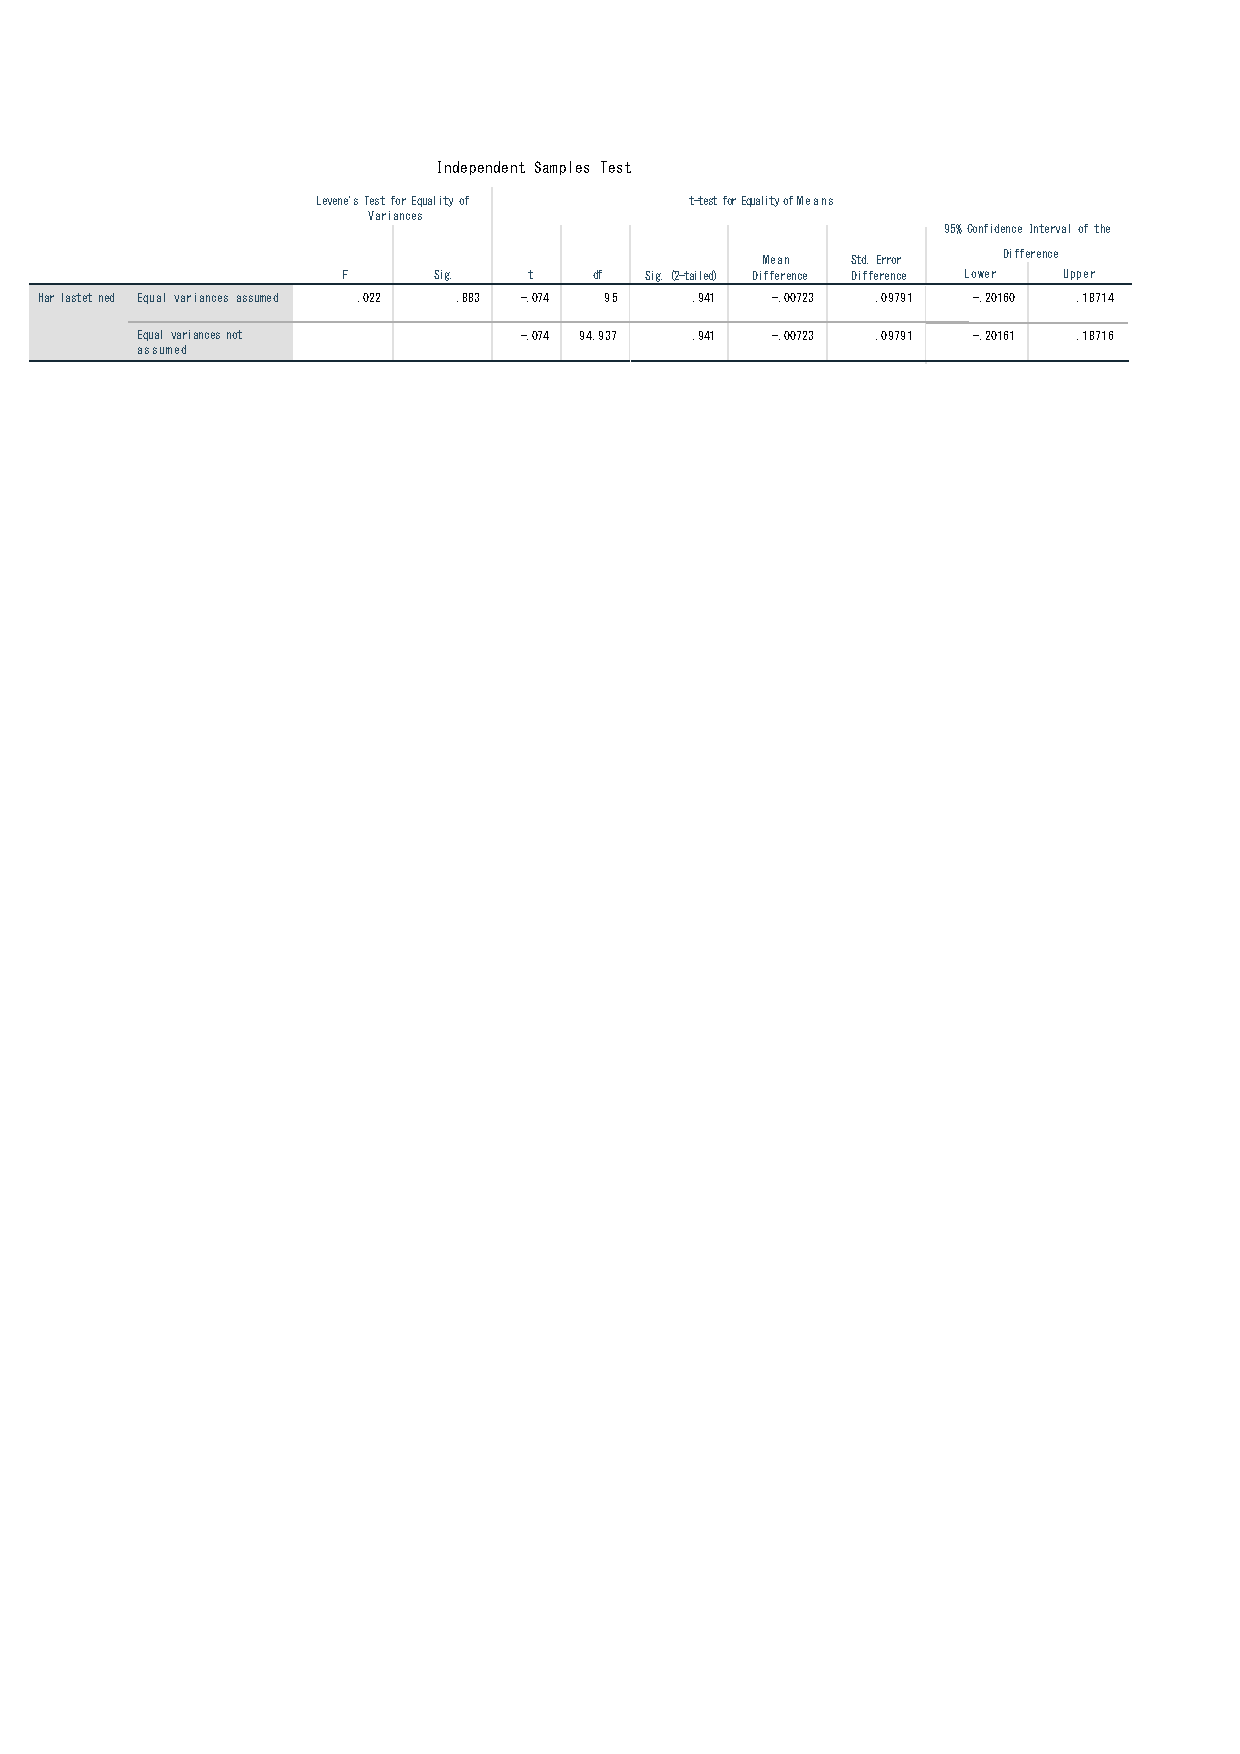
\includegraphics[scale=0.7]{case_1/bilder/studentby_lasterned_ttest.pdf}
    \caption{Independent Samples Test av studentbyer opp mot om de laster ned eller ikke}
    \label{fig:studby_lasterned_ttest}
\end{figure}

Dette betyr at det er ingen forskjeller på personer som bor på Kallerud og de som bor på andre studentbyer når det kommer til om de laster ned, til tross for ti ganger så rask nedlasting og opplasting. 

\subsection{ANOVA-analyse}
I denne analysen ser vi på forskjeller mellom IT fakultetet og de andre fakultetene i henhold til svarene som ble gitt på påstandene. Det ble i tillegg også kjørt analyser basert på kjønn og alder, men med alder var datafordelingen for lav på enkelte alternativer til å kunne si noe om det så den har uteblitt i rapporten. På kjønn brukte vi ANOVA til å se forskjeller i svar på påstandene og kjennskap til IT reglement. Bare kjennskap til IT reglement vises her siden det var det eneste med både tilstrekkelig svar fra hvert kjønn og signifikans i forskjellen.

%-----------------------------------------------ONEWAY ANOVA - fakultet MOT PÅSTAND------------------------
%-----------------------------------------------DESCRIPTIVES------------------------------------------------
\begin{figure}[H]
    \centering
    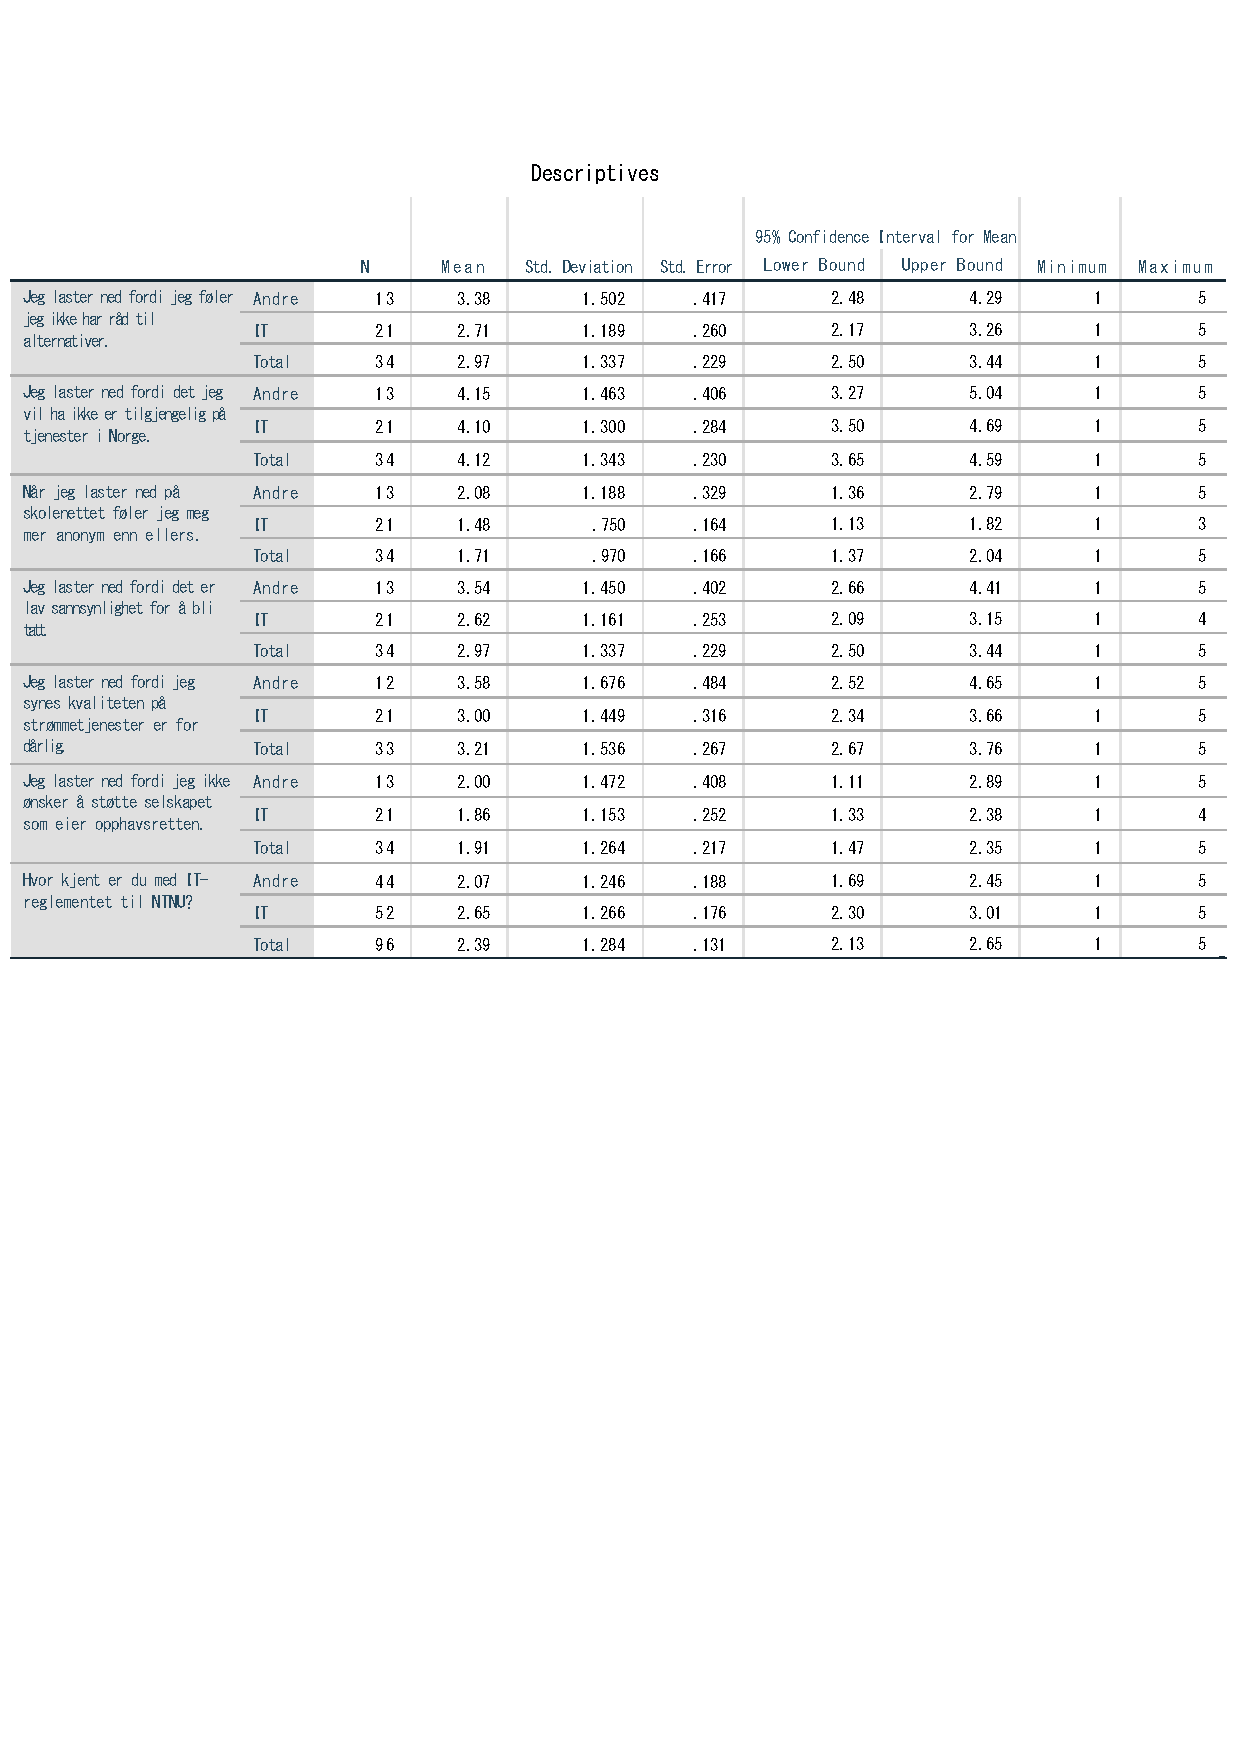
\includegraphics[scale=0.6]{case_1/bilder/fakultet_pastander_descriptive.pdf}
    \caption{Descriptives for IT fakultetet og de andre fakultetene når det kommer til påstander}
    \label{fig:fakultet_pastander_descriptive}
\end{figure}

%-----------------------------------------------ANOVA-------------------------------------------------------
\begin{figure}[H]
    \centering
    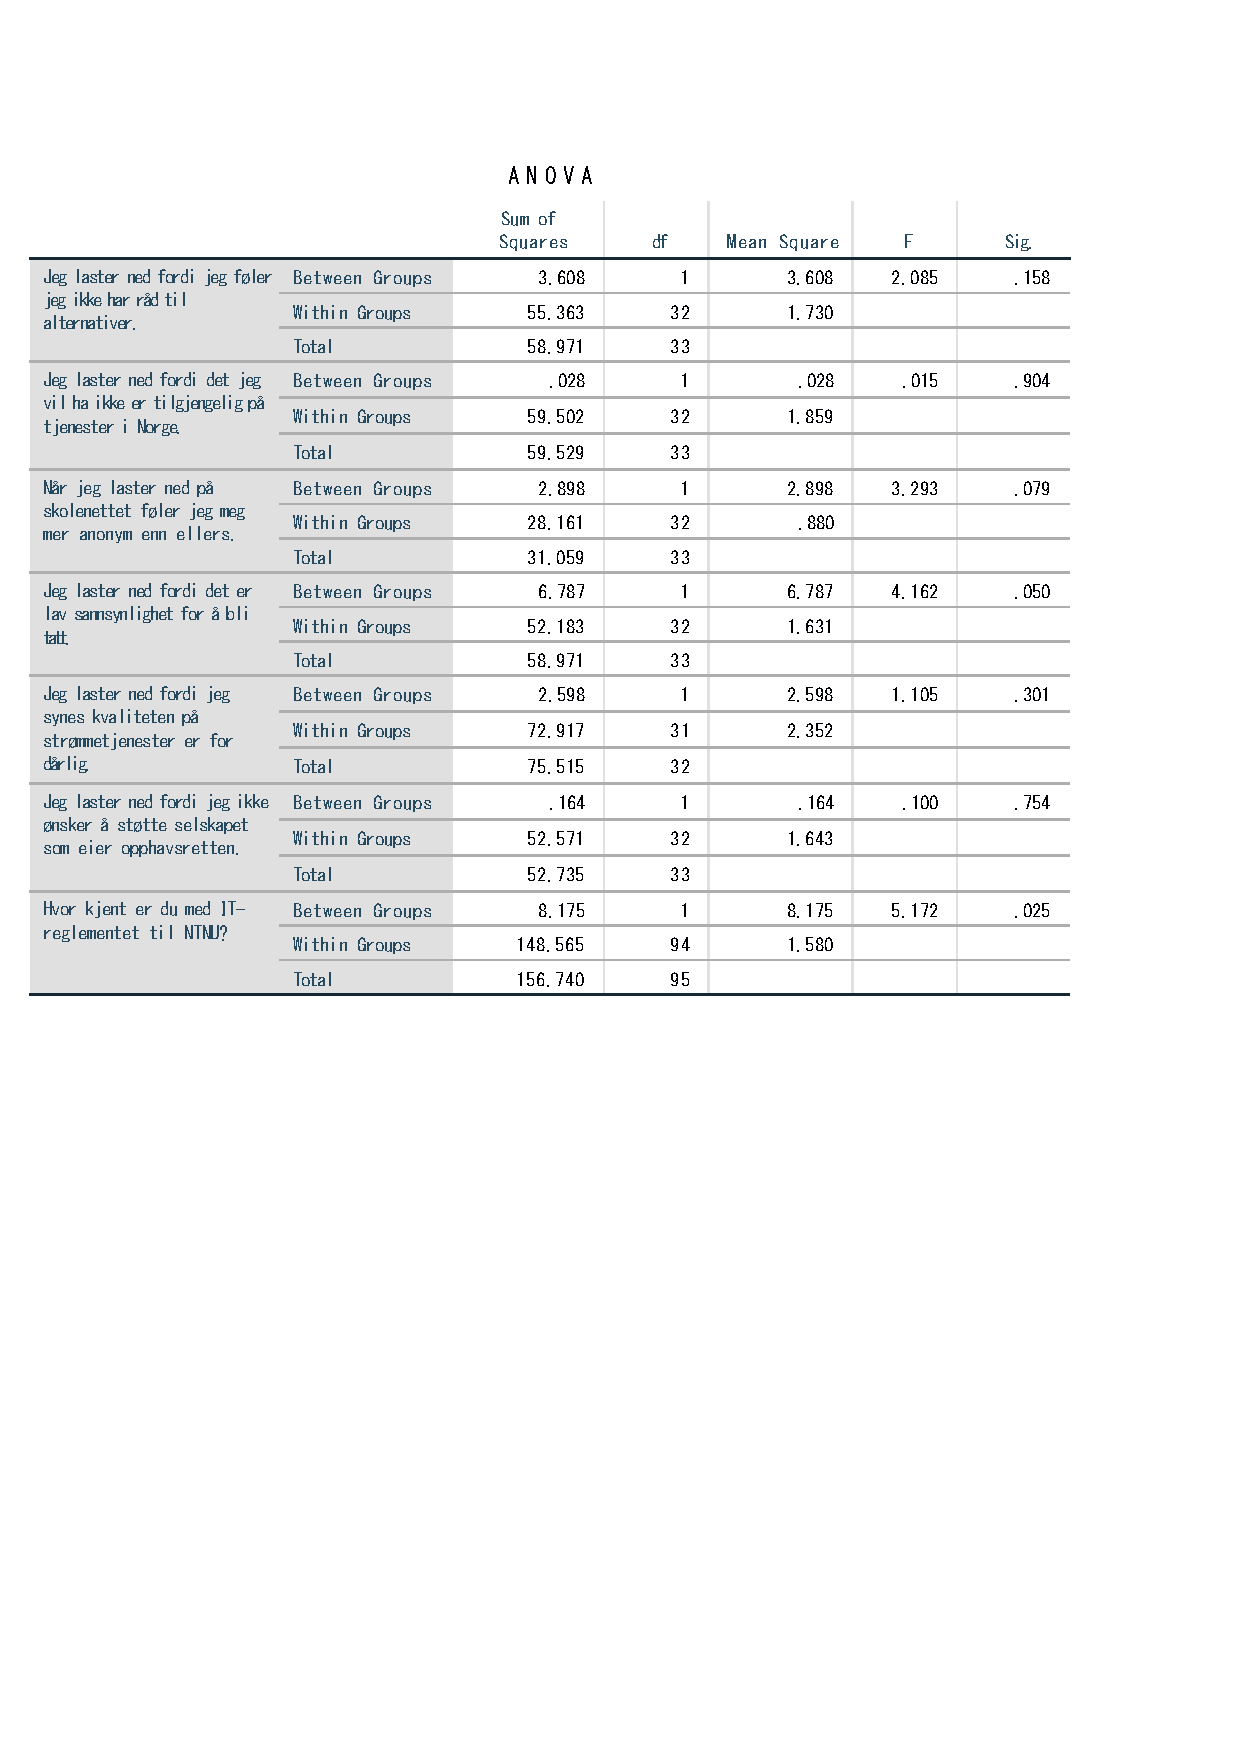
\includegraphics[scale=0.7]{case_1/bilder/fakultet_pastander_anova.pdf}
    \caption{Forskjellen mellom IT fakultetet og de andre fakultetene når det kommer til påstander}
    \label{fig:fakultet_pastander_anova}
\end{figure}

Det viser seg å være signifikant forskjell på IT og de andre fakultetene når det kommer til lav sannsynlighet for å bli tatt og kjennskap til IT reglement. Respondenter fra IT fakultetet er mer uenig i at de laster ned på grunn av lav sannsynlighet for å bli tatt (sig. 0,050), og de kjenner også IT reglementet bedre (sig. 0,025). 

%-----------------------------------------------DESCRIPTIVES------------------------------------------------
\begin{figure}[H]
    \centering
    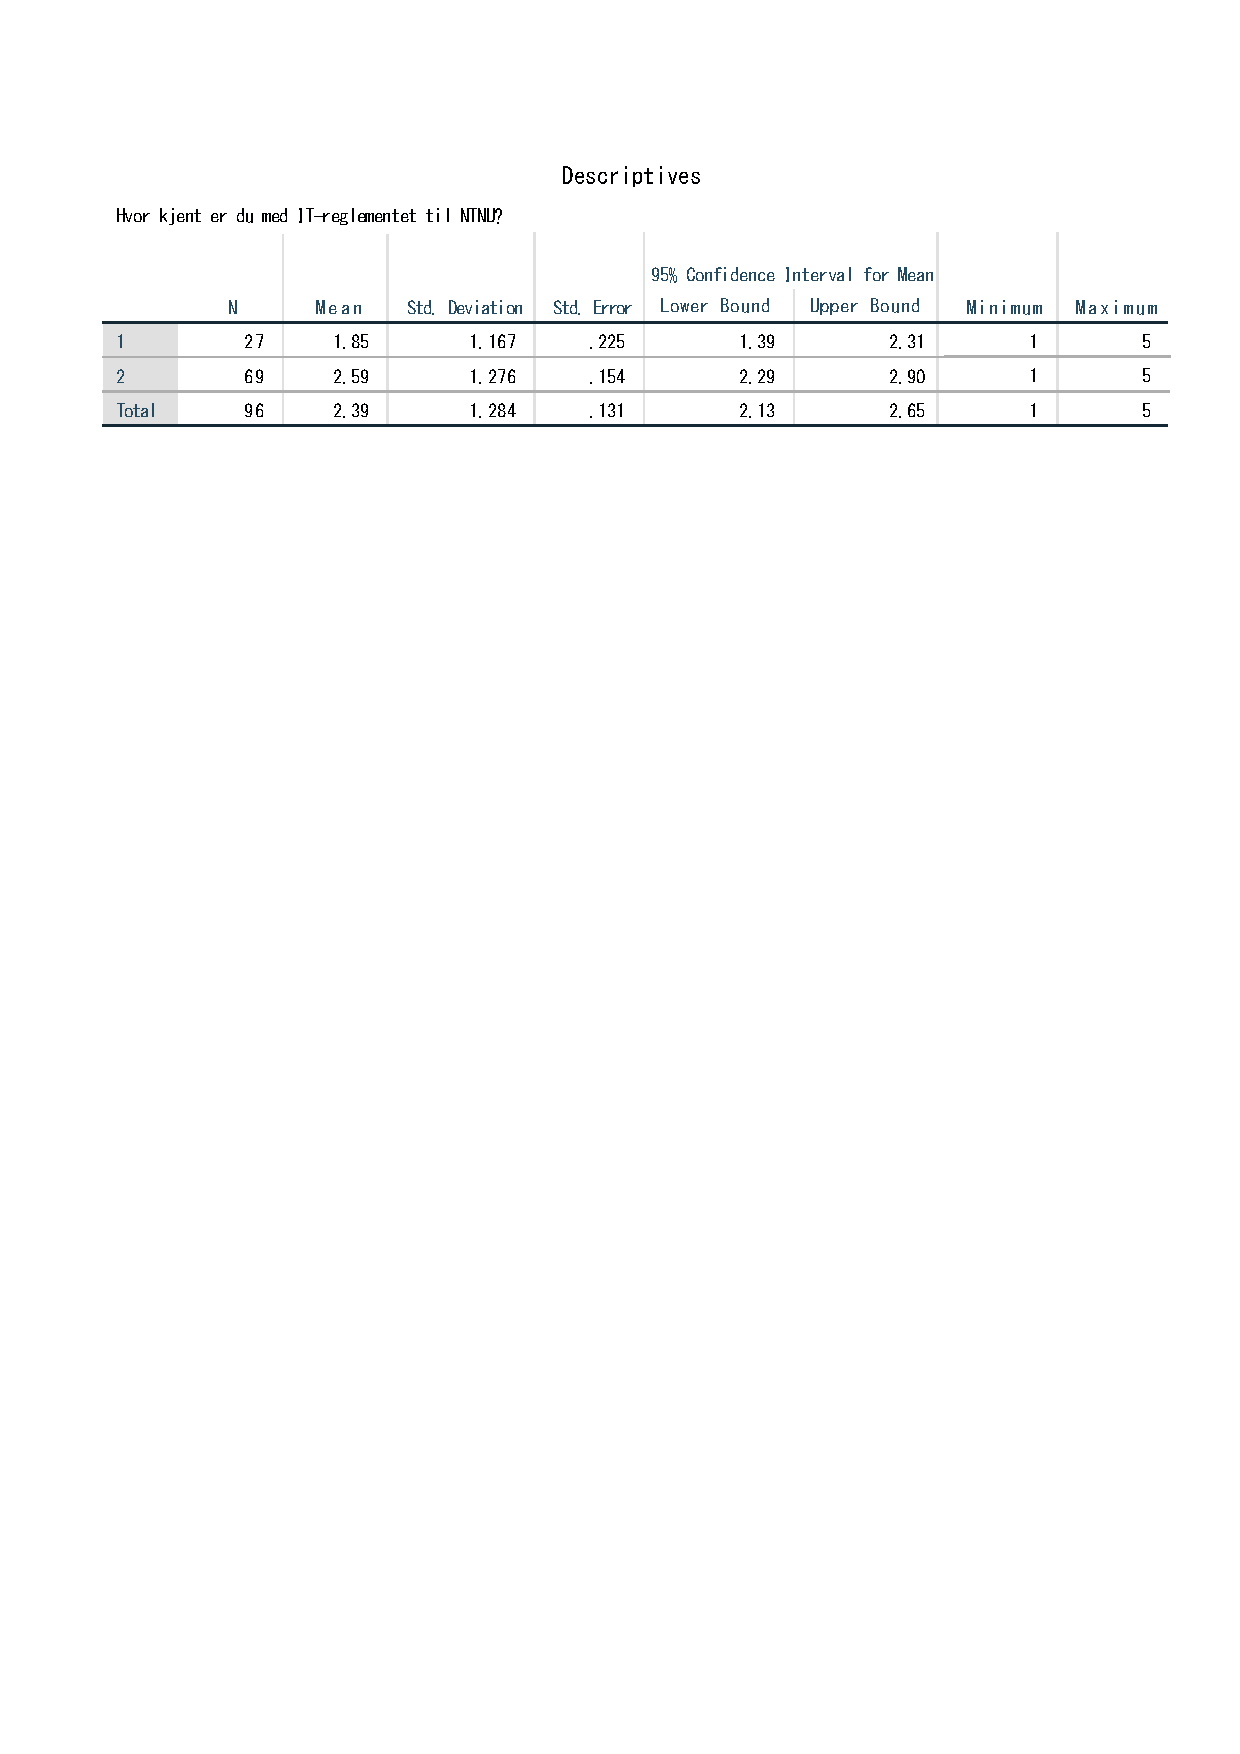
\includegraphics[scale=0.6]{case_1/bilder/kjonn_kjent_descriptive.pdf}
    \caption{Descriptives for kjønn når det kommer til kjennskap til IT reglement}
    \label{fig:fakultet_pastander_descriptive}
\end{figure}

Kvinner er 1 og menn er 2 i disse tabellene.
%-----------------------------------------------ANOVA-------------------------------------------------------
\begin{figure}[H]
    \centering
    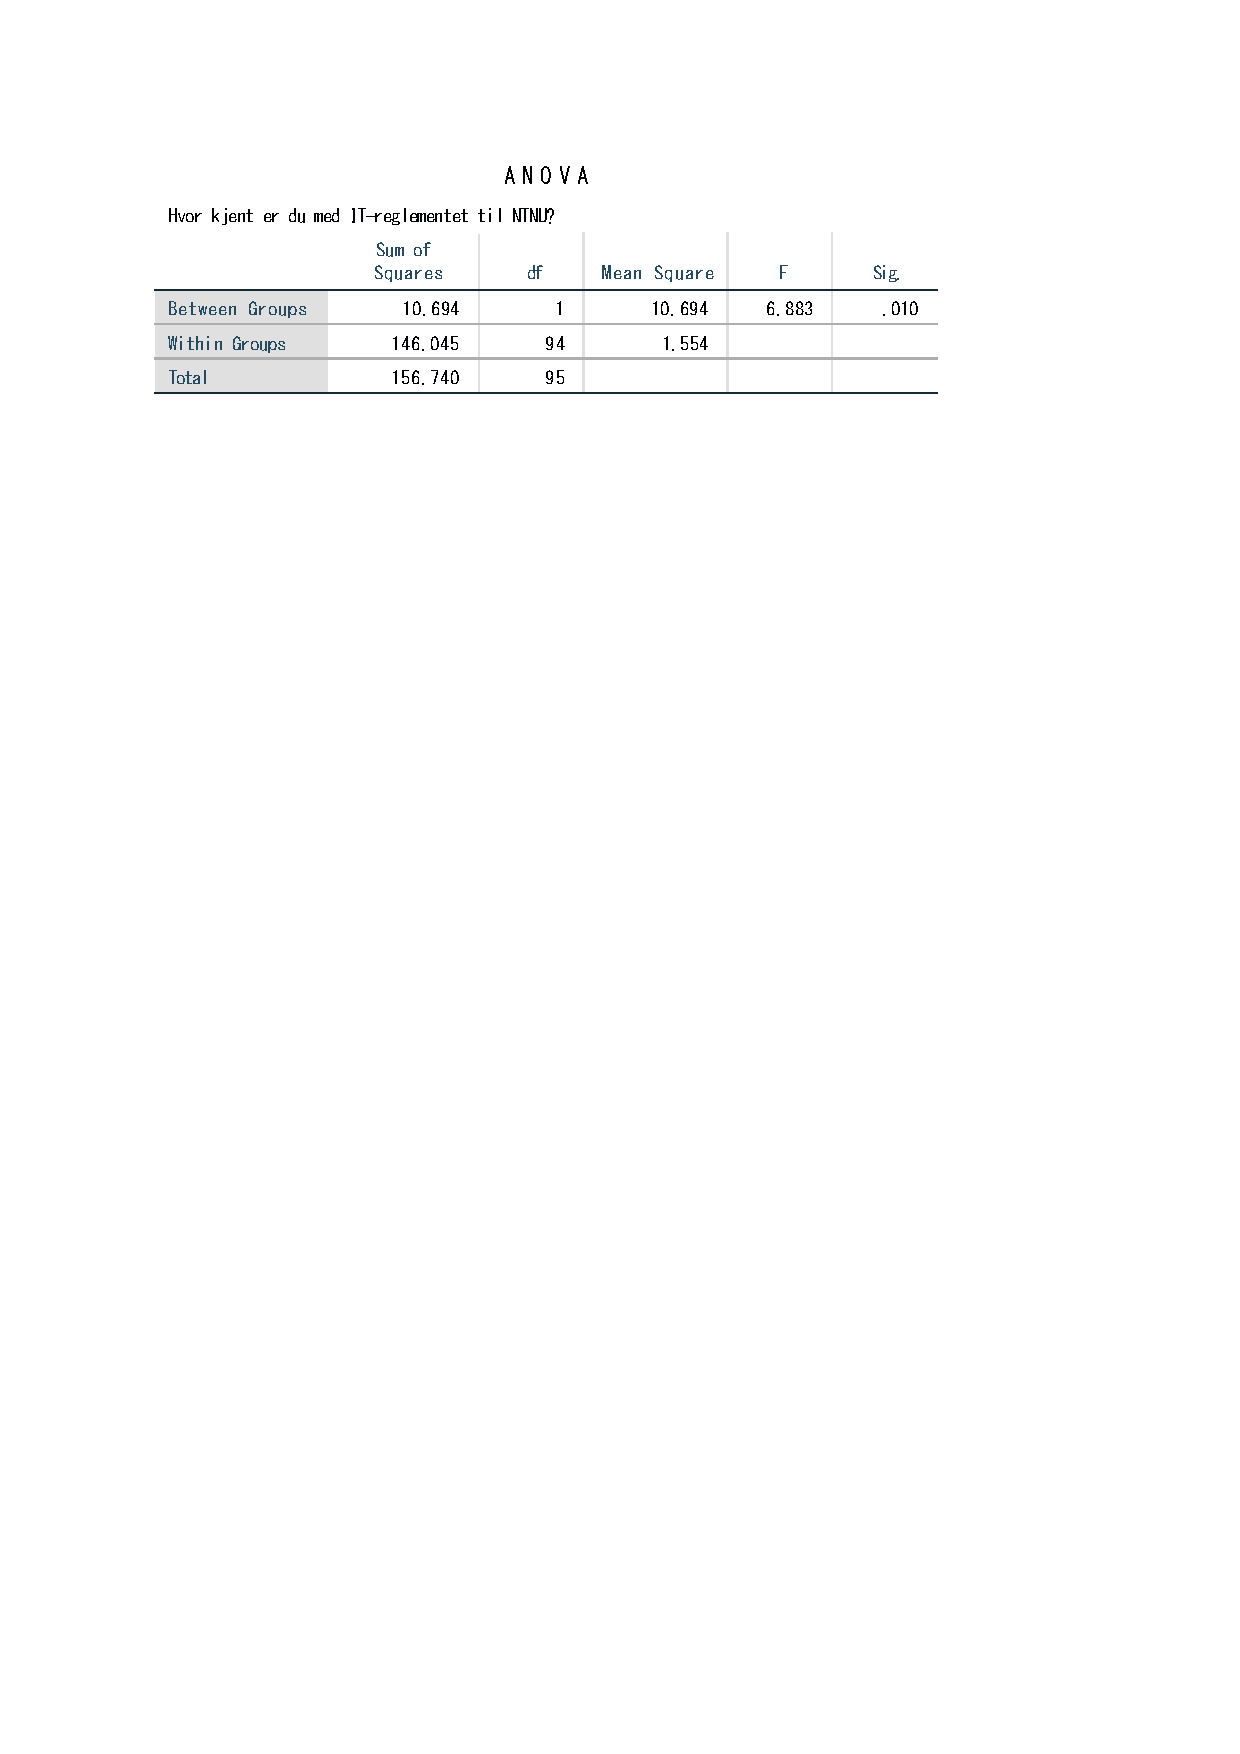
\includegraphics[scale=0.7]{case_1/bilder/kjonn_kjent_anova.pdf}
    \caption{Forskjellen mellom kjønnene når det kommer til kjennskap til IT reglement}
    \label{fig:fakultet_pastander_anova}
\end{figure}

I tabellen over ser vi at menn svarer at de har generelt sett bedre kjennskap til IT reglementet, selv om vi fra tidligere vet at menn er overrepresentert i de som laster ned ulovlig. Noe av det kan forklares med at IT studenter stort sett er menn, og de kjenner reglementet bedre. 

\subsection{Konklusjon av verktøy}
Statistisk analyse var tidkrevende å sette seg inn i for oss som ikke har hatt statistikk fra før. Noe av det var også krevende fordi vi ikke hadde godt nok datagrunnlag til å gjøre alt vi ville. Ellers fungerte det greit til å finne et par signifikante forskjeller i demografien. 

%------------------------------------------------------------------------------------------------------------------------

\section{Affinitetsdiagram}
Affinitetsdiagram brukes til å analysere data som det ikke er mulig å nummerere, eksempelvis meninger eller ideer. Affinitetsdiagram grupperer data og finner de underliggende korrelasjoner og likhetstrekk i gruppen. 

\subsection{Ønsket utbytte}
Ønsket utbytte av affinitetsdiagramet er å få en oversikt over hva deltakerne mener skal til for at de vil stoppe med fildeling.
\subsection{Gjennomføring og resultater}
I spørreundersøkelsen spurte vi om hva som skal til for at deltagerne vil slutte med fildeling. Svarende vi fikk ble sortert inn i 16 grupper organisert under fire hovedkategorier. Hvis noen av deltakere har kommet med flere forslag har hvert av forslagene fått en stemme.  

\begin{figure}[H]
    \centering
    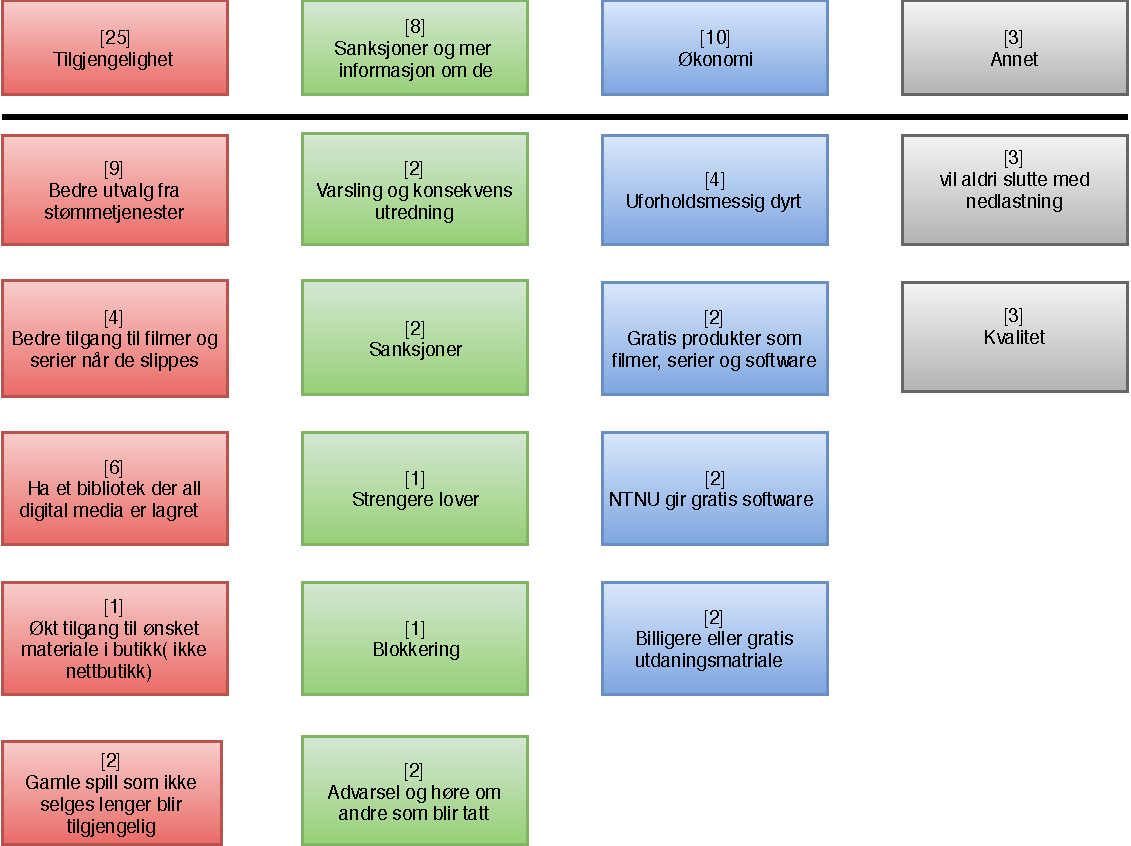
\includegraphics[scale=0.6]{case_1/bilder/stoppe_nedlastning.pdf}
    \label{fig:stoppe_nedlastning}
    \caption{Hva skal til for at personer vil slutte med nedlasting?}
\end{figure}

Denne analysen gir oss ikke rotårsaken til at studenter laster ned, men kan brukes til å gi pekepinne på hva studenter mener skal til for at de vil slutte med nedlasting. Vi kan se på affinitetsdiagram at det er virker å være tre grunner til at personer laster ned. Der det å gjøre materiale mer tilgjengelig virker som den beste løsningen for å stoppe personer fra å nedlaste. Dette samsvarer med de tidligere funnene i figur \hyperref[fig:tilgjengelighet]{Tilgjengelighet}. Problemet med tilgjengelighet er at det er et mer global problem, basert på at en del av de tradisjonell media bruker forsatt geografiske begrensinger. Så da har vi igjen kategoriene økonomi og sanksjoner. Ser man på saksjoner så er det flere som mener at det å være mer vokal om konsekvenser og andre som blir tatt kan være et godt tiltak, som er tildels motstridende med tidligere figur om \hyperref[fig:konsekvens_lasterned]{Konsekvens av å laste ned}. På økonomi eksisterer det et flertall som mener at de har ikke har noe imot å betale for produktet så lenge de mener det er rimelig. Og et mindretall som vil ha gratis produkter. Her kan NTNU kanskje gjøre noe i form av muligens studentrabatter eller de betaler for produktet.          


\subsection{Konklusjon av verktøy}
Affinitetsdiagram er et vektøy som ikke har sin rot i matematikk eller statistikk, men er heller et mer kreativ verktøy der brukerne bruker sin egen tankegang til å finne de korrelerende gruppene. Dette fungerer bra når dataene man henter er på to forskjellige språk og der deltakerne varierer hvor mye de skriver. Siden dataene er blitt organisert inn i grupper er det mye lettere å analysere hva personene mener er viktig. Det negative med affinitetsdiagram er risikoen for at forslag blir gruppert feil eller at det gjøres en feil korrelasjon.        
  

\section{Konklusjon av dataanalysen}
Her diskuteres de funnene som er blitt gjort etter å ha analysert dataene fra spørreundersøkelsen. 

\subsection{Omfang}
Det var 35\% som svarte de hadde lastet ned opphavsrettsbeskyttet materiale i hybelen før, mens 65\% ikke hadde gjort det. Dette var noe lavere enn vi hadde trodd, men omfanget er fortsatt stort og svært problematisk fra skolen sin side. Vi har også sett at de fleste laster ikke ned så veldig ofte. I løpet av en måned laster de fleste ned bare en til tre torrents, eller ingenting i det hele tatt. Allikevel er det i tillegg en god del folk som laster ned over ti torrents i løpet av en måned. Dette vil si at enten så er du en småforbruker eller en storforbruker, det er veldig få i midten, men det er flest av småforbrukerne som vist i figur \ref{fig:antalltorrents}.

\subsection{Demografiske forskjeller og særtrekk}
Gjennom analysen fant vi en rekke forskjeller og særtrekk for de demografiske kategoriene. Det er altså snakk om særtrekk og forskjeller mellom kjønn, fakultet, alder og studentby som er relevant. Alder ble ikke sett så mye på siden litt over 74\% av de spurte var mellom 20 og 25, og vi hadde ikke nok data på de andre som vist i tabell \ref{tab:alder}. 

\subsubsection{Kjønn}
Av de 97 respondentene var det 70 menn og 27 kvinner, altså henholdsvis 72,2\% og 27,8\%. Mellom kjønnene var det store forskjeller på om de hadde lastet ned ulovlig eller ikke. Hos menn var det nesten dødt løp på de som laster ned og de som ikke gjør det, 44.3\% svarte at de hadde lastet ned. Hos kvinner derimot var det bare 11\% som svarte de hadde lastet ned ulovlig på hybelen før. Menn kjenner til IT reglementet noe bedre enn kvinner. 

\subsubsection{Fakultet}
Antall respondenter i de ulike fakultetene var ganske spredt. Det var en sterk overvekt av IT-studenter som svarte på undersøkelsen. Det var 50.5\% av personene som tilhørte Fakultetet for informasjonsteknologi og elektroteknikk. Dette er litt mer enn de andre fakultetene til sammen så vi valgte å ta utgangspunkt i IT fakultetet i forhold til de andre fakultetene siden vi regnet med at det ville være en forskjell der. Og det var det også, studenter tilhørende IT fakultetet har større andel nedlastere enn andre fakulteter. Vi fant også ut at IT studentene hadde bedre kjennskap til IT reglementet enn de andre, selv om de laster ned mer.

\subsubsection{Studentby}
Selv om Kallerud studentby har ti ganger så raskt nett som de andre studentbyene, kan vi ikke vise til noen signifikante resultater som sier det fører til flere som laster ned. Anova-analysen viser at studenter fra Kallerud og de andre studentbyene så og si er likt representert i de som laster ned.

\subsection{Dårlig tilgjengelighet på tjenester}
Dette var hovedfunnet vårt fra histogrammene. Det viste seg at tilgjengelighet på tjenester var en veldig stor grunn til at de fleste valgte å laste ned. Det var bare 4 (11,8\%) som svarte at dette i liten grad betydde noe for dem. Enda færre svarte at de var litt uenig eller nøytral til påstanden, nemlig bare 1 (2,9\%) på hver. Det var derimot 9 (26,5\%) som svarte at de var litt enig, og hele 19 som svarte at de var i stor grad enig med påstanden. Det tilsvarer 55,9\%.
I tillegg til dette ville vi undersøke om de hadde grunnlag til å si dette. Vi laget et histogram som klynget sammen påstanden om tilgjengelighet med hvor mange videostrømmingstjenester de hadde tilgang på. Det var ikke så mange som hadde svart at de var i liten grad enig med påstanden, så datagrunnlaget for å si noe om hvor mange tjenester de som sa seg uenig hadde var vagt.Det viste seg derimot at de som sa seg enig i påstanden også hadde svært mange strømmetjenester, noe som sier at det som er tilgjengelig i Norge ikke er nok til å få dem til å slutte å laste ned. 
I affinitetsdiagrammet var det mange som også så på tilgjengelighet som det store problemet når det kom til hvordan de ville løse det. 25 personer ville stoppet å laste ned hvis det ble gjort noe med tilgjengeligheten. 

\subsection{Alternative tjenester for dyrt i forhold til hva du får}
Respondentene svarer ganske spredt på at de laster ned fordi de føler de ikke har råd til alternativer. I tillegg til det svarer ti stykker i affinitetsdiagrammet at de hadde stoppet å laste ned dersom det ikke var uforholdsmessig dyrt eller hvis noen hadde tilbudt gratis tjenester. Siden det også er mange som ikke bryr seg om økonomien når det kommer til nedlasting er ikke dette funnet like relevant som tilgjengeligheten, men det er verdt å ta i betraktning. Dette var overraskende siden vi hadde trodd dette betydde mye mer for folk enn det egentlig gjør. 

\subsection{Dårlig håndhevelse og kommunikasjon av eksisterende lover}
I undersøkelsen svarte 47.4\% at de ikke kjente til konsekvenser ved brudd på opphavsretten. Det viser seg også at generelt sett de som laster ned kjenner konsekvensene bedre enn de som ikke gjør det. Dette viser at selv om de kjenner til konsekvensene laster de ned uansett fordi sjansen for å bli tatt for det er tilnærmet null. Det var også svært få som kjente til NTNU's IT reglement, som blant annet viser til norske lover angående krenking av opphavsrett og ulovlig fildeling. Sanksjoner for brudd på reglementet kan være utestengelse av nettet i opptil fem dager, men driftsansvarlige er dårlige til å håndheve disse reglene, selv om det er krav om det i reglementet \cite{ITReg}. 
\chapter{Rotårsaksidentifisering}
Arbeidet i denne fasen går ut på å identifisere rotårsaken. I foregående fasen ble en rekke mulige årsaker identifisert og analysert, men nå er det tid for å finne den faktiske rotårsaken. Det er mange forskjellige verktøy som kan brukes i denne fasen, men vi har valgt oss en type årsak-virkning diagram for vårt utgangspunkt.

\section{Årsak-virkningsdiagram}
Et årsak-virkning diagram er et diagram som analyserer forholdene mellom et problem og dets årsaker. Det kombinerer aspekter ved idémyldring med systematisk analyse. Det finnes to typer årsak-virkning diagrammer, fiskebeindiagram og prosessdiagram. Mens et prosessdiagram er mer direkte fokusert på problemet på innsiden av forretningsprosessene, er et fiskebeindiagram en mer generell tilnærming for å adressere alle potensielle årsaker\cite{RCA}. Fiskebeindiagram passer best i dette caset.

\subsection{Ønsket utbytte}
Ved bruk av dette verktøyet ønsker vi å sitte igjen med en visuell fremstilling av rotårsaken til problemet. Dette vil gjøres ved å identifisere hva som skaper årsakene vi har funnet fram til i foregående fase.

\subsection{Gjennomføring}
Det er anbefalt å bruke en tusjtavle for å tegne opp fiskebeindiagrammet, men vi valgte å bruke et nettbasert program som er laget for å skape diagrammer med flere brukere involvert i sanntid. De hadde en egen mal for fiskebeindiagram som vi valgte å gå ut fra. Stegene vi fulgte i prosessen er hentet fra boka om rotårsaksanalyse \cite{RCA} og ble som følger:
\begin{enumerate}
    \item Vi beskrev problemet klart og tydelig
    \item Vi tegnet opp problemet på slutten av fiskebeindiagrammet
    \item Vi identifiserte hovedkategoriene av årsakene til problemet og tegnet det opp på fiskebeinene i diagrammet
    \item Vi idémyldret alle mulige årsaker i hver kategori, en kategori om gangen, og skrev det inn i diagrammet fortløpende
    \item Til slutt analyserte vi de identifiserte årsakene og bestemte de mest sannsynlige rotårsakene
\end{enumerate}

\subsection{Resultater}
Vi beskrev problemet som ulovlig fildeling på skolenettet etter tittelen på caset. Hovedkategoriene vi ønsket å utforske har vi basert på dataanalysen i forrige fase for å finne de mest relevante. Disse var etter vår mening Økonomi, Risiko og Tilgjengelighet. Idémyldringen var i stor grad basert på data og funn fra analysen, med innslag fra den første idémyldringen og andre nye idéer som dukket opp.

\begin{figure}[H]
    \centering
    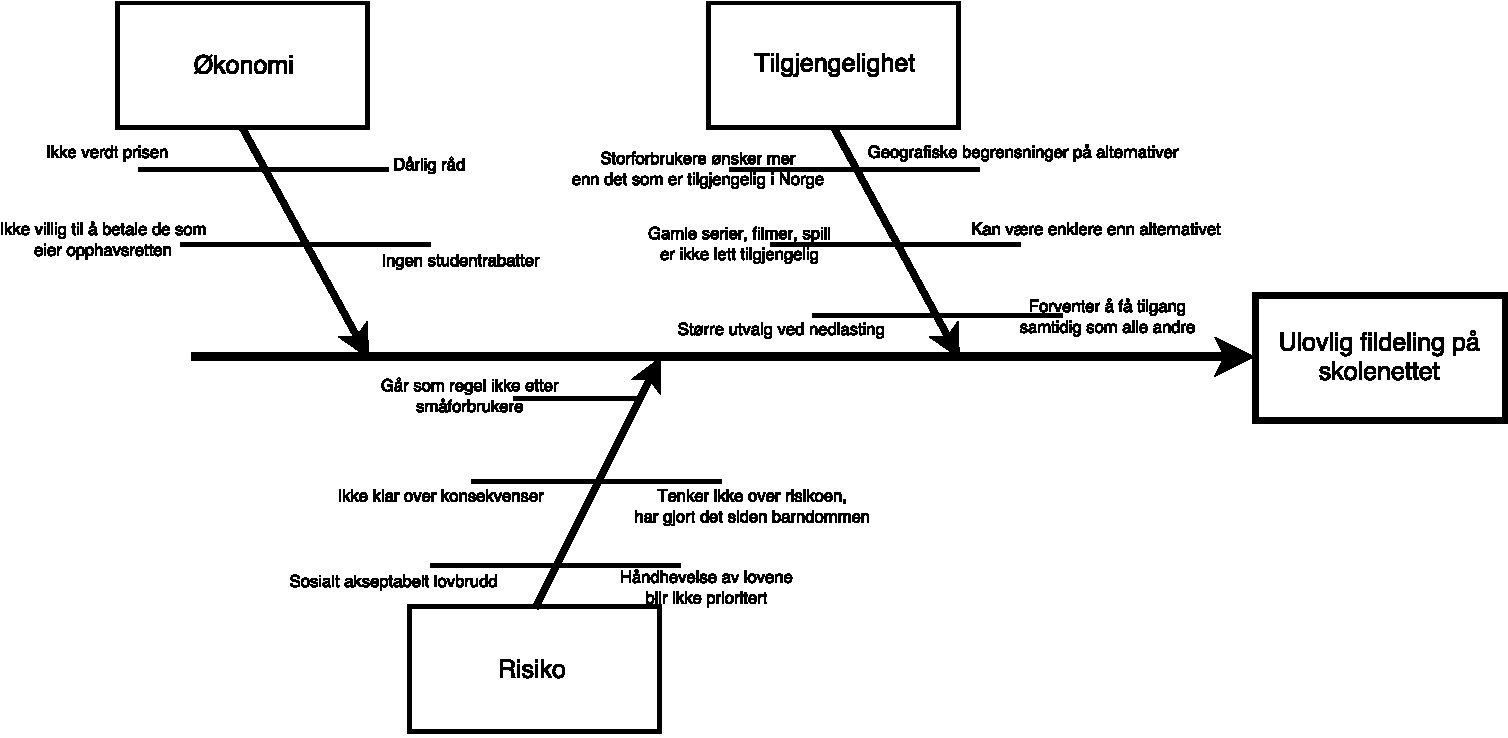
\includegraphics[scale=0.5]{case_1/bilder/fiskebein.pdf}
    \label{fig:fiskebein}
    \caption[Fiskebein]{Fiskebeindiagram over hovedkategorier og årsaker}
\end{figure}

Etter videre analyse av figuren har vi kommet fram til at rotårsaken til fildeling er en kombinasjon flere faktorer, men én skiller seg ut, nemlig tilgjengelighet. Med tilgjengelighet mener vi spesifikt at folk bedriver ulovlig fildeling fordi det er dårligere utvalg på alternative tjenester i Norge. Det finnes også noen mindre årsaker som påvirker folk til å laste ned. Blant dem er at mange føler tjenestene ikke er verdt prisen de må betale når de bare får tilgang på en begrenset mengde materiale. Den siste årsaken går på at håndheving av lovene knyttet til ulovlig fildeling ikke blir prioritert, og derfor har skapt en kultur der det er sosialt akseptabelt å laste ned. Rotårsakene er listet etter viktighet der den første er hovedårsaken:

\begin{enumerate}
    \item Dårligere utvalg på alternative tjenester i Norge
    \item Tjenestene er ikke verdt prisen
    \item Håndheving og kommunisering av lovene knyttet til ulovlig fildeling blir ikke prioritert
\end{enumerate}

\subsection{Konklusjon av verktøy}
Verktøyet fungerte som en strukturert måte å kategorisere alle mulige rotårsaker vi hadde kommet fram til i tidligere faser. Det var også mulighet for å inkludere andre mulige årsaker som vi hadde i tankene gjennom prosessen. Det kan kanskje i noen sammenhenger være vanskelig å kategorisere de ulike årsakene dersom disse gruppene ikke er klart definert på forhånd, men i denne sammenhengen var det veldig intuitivt. Det kan også hende idémyldringen blir litt for fokusert på de ulike kategoriene siden man definerer disse på forhånd. Ellers et veldig godt verktøy som ga oss relevante resultater. 
\chapter{Rotårsakseliminering}
Arbeidet i denne fasen går ut på å finne løsninger for å eliminere rotårsaken. I denne fasen har vi valgt å bruke vektøyet seks tenke hatter og SIT for å finne de beste måtene å få eliminert rotårsaken på. 

\section{De seks tenkehattene}
De seks tenkehattene er et diskusjons verktøy, som går ut på at man gir personer forskjellige hatter/roller til prossessen. De forskjellige rollene er som følger:
\begin{description}
    \item [Hvit hatt] kynisk, faktabasert og systematisk.
    \item [Rød hatt] er den emosjonelle personen, han som følger magefølelsen og egen intuisjon
    \item[Svart hatt] pessimistisk og negativ, fokuserer på hvordan idéen ikke vil
    fungere
    \item [Gul hatt] optimistisk og positiv, fokuserer på hva som skal til for at løsningen skal kunne fungere
    \item[Grønn hatt] fokuserer på kreativitet og skal prøve å bygge på idéer
    \item[Blå hatt] assosieres med himmelen, og skal se problemet fra et større perspektiv.
\end{description}

\subsection{Ønsket utbytte}
Ønsket utbytte med bruk av seks tenkehatter, er å skape en forståelse rundt rotårsaken og komme opp meg mulige tiltak for å eliminere problemet. Siden problemet virker vanskelig å fikse fra skolen sin side måtte vi komme med noen kreative løsninger, og de seks tenkehattene fungerer godt for dette.

\subsection{Gjennomføring}
Siden vi bare var fire tok to av oss på seg to hatter og resten en. Så startet vi å diskutere problemstillingen og hvordan vi burde gå inn for å eleminere rotårsaken, vi kom frem til en rekke mulige løsninger. Etter at vi var ferdig med de seks tenkehattene gikk vi fort igjennom de forskjellige forslagene, for å se på hva som var praktisk gjennomførbare og ikke, på slutten av prosessen tok vi altså å brukte de to siste punktene fra SIT, for å luke ut de beste forslagene, og for å bestemme oss for hva som var gjennomførbart

\subsection{Resultater}
Ut i fra prosessen med de seks tenkehattene kom vi fram til både gjennomførbare og ikke gjennomførbare tiltak. 
\subsubsection{Gjennomførbare tiltak}
\begin{itemize}
    \item Tilby produkter fra selskap som skolen får flest notifikasjoner fra
    \item Stenge torrentprotokollen for alle på nettverket.
    \item Grense på nedlastning og opplastning av data.
    \item Være strengere når det gjelder oppfølging av IT-reglementet. 
    \item Bytte ISP til studentboligene.
    \item Oppmerksomhetskampanje om konsekvenser.
    \item Avtale med kino for billige/gratis nye filmer
\end{itemize}

\subsubsection{Ikke gjennomførbare tiltak}
\begin{itemize}
    \item Alt av materiale blir gratis og tilgjengelig på ett samlet sted
    \item Fjerne geografiske blokkeringer
\end{itemize}

Noen av disse vil ikke være gjennomførbare for NTNU så vi har valgt å ikke ta de med videre til implementering, men vi følte de kunne være interessante å nevne. Av de 11 forslagene er det kun 4-5 vi mener har høy sannsynlighet for å bli kvitt rotårsaken, helt eller delvis, eller flytter rotårsaken vekk fra NTNU ansvarsområde. Etter videre vurdering har vi kommet fram til de mest lovende løsningene for å fjerne rotårsaken: 

\subsubsection*{Tiltak som fjerner rotårsaken til at folk laster ned}

\begin{enumerate}
    \item Alt av materiale blir gratis og tilgjengelig på ett samlet sted
    \item Fjerne geografiske blokkeringer
    \item Tilby produkter fra selskap som skolen får mest notis fra
    \item Prøve for studenter for å få full hastighet på nettverk
\end{enumerate}

\subsubsection*{Tiltak som fjerner rotårsaken til at skolen får notifikasjon fra opphavsrettshaverne}

\begin{enumerate}
    \item Bytte ISP til studentboligene
    \item Stenge torrentprotokollen for alle på nettverket
\end{enumerate}

Rotårsaken til at folk bedriver ulovlig fildeling er ikke et problem som lett kan løses av skolen. Vi har gitt et par forslag til hva som kan fjerne rotårsaken helt, men av disse er ikke alle gjennomførbare for skolen. Vi har også foreslått et par tiltak som ikke fjerner rotårsaken og noen som fjerner rotårsaken til hvorfor folk laster ned. De tiltaken som ikke fjerner rotårsaken vil flytte rotårsaken bort fra NTNU's ansvarsområde.

\subsection{Konklusjon av verktøy}
Verktøyet fungerte godt til å starte en diskusjon rundt elimineringsalternativer, men det utviklet seg fort til en form for idémyldring, siden det var vanskelig å forholde oss til de forskjellige sinnstilstandene/hattene. Det var også et par komplikasjoner siden to av oss måtte ha to hatter samtidig. Ellers var det en kreativ og morsom prosess der mange gode alternativer kom fram. 

\section{Systematisk Innovativ Tenkning (SIT)}
Systematic Inventive Thinking inneholder fem hovedprinsipper:

\begin{enumerate}
    \item \textbf{Attributtavhengighet} Endre på en essensiell variabel.
    \item \textbf{Komponentkontroll} Ser på hvordan et produkt er tilknyttet omgivelsene sine.
    \item \textbf{Erstatning} Bytte ut en del av produktet med noe i omgivelsene til produktet.
    \item \textbf{Forkastning} Fjerne en del av produktet for å bedre det.
    \item \textbf{Oppdeling} Prøver å splitte et produkts attributter i to.
\end{enumerate}

\subsection{Ønsket utbytte}
Ved å bruke SIT metoden ønsker vi å få kreative løsninger på hvordan vi kan stoppe ulovlig nedlasting.

\subsection{Gjennomføring}

\subsubsection{Komponenter} Alle komponenter blir listet.

\begin{itemize}
    \item Lite kunnskap om konsekvenser
    \item Raskt internett
    \item Alt er tilgjengelig samtidig overalt
    \item Økonomi
  %  \item Kjedsomhet - laste ned serier/spill for å ha noe å gjøre
\end{itemize}

\subsubsection{Idémyldring med SIT hovedprinsipper} I dette steget ble SIT prinsippene brukt til å finne løsninger til komponentene i det foregående steget.

\paragraph{Lite kunnskap om konsekvenser}
\begin{itemize}
    \item \textbf{Attributtavhengighet} Løfte opp kunnskapen om konsekvenser og lover.
    \item \textbf{Komponentkontroll} Ha en test for å se at folk forstår IT-reglementet og mulig kursing.
    \item \textbf{Erstatning} Ikke gjennomførbart
    \item \textbf{Forkastning} Ikke gjennomførbart
    \item \textbf{Oppdeling} Ikke gjennomførbart
\end{itemize}

\paragraph{Raskt internett som skolen eier}
\begin{itemize}
    \item \textbf{Attributtavhengighet} Sperre torrenting protokollen.
    \item \textbf{Komponentkontroll} Ikke gjennomførbart.
    \item \textbf{Erstatning} Ha tregere internett, slik at folk ikke laster ned hjemme.
    \item \textbf{Forkastning} Fjerne internett fra Sit boligene/bytte ISP.
    \item \textbf{Oppdeling} Ikke gjennomførbart
\end{itemize}

\paragraph{Tilgjengelighet}
\begin{itemize}
    \item \textbf{Attributtavhengighet} Få rettighethaverne til å samle alt innhold til ett sted 
    \item \textbf{Komponentkontroll} Ikke gjennomførbart.
    \item \textbf{Erstatning} Tilby gratis filmer/serier og spill.
    \item \textbf{Forkastning} Ikke gjennomførbart
    \item \textbf{Oppdeling} Ikke gjennomførbart
\end{itemize}

\paragraph{Økonomi}
\begin{itemize}
    \item \textbf{Attributtavhengighet} Mer penger fra lånekassen. 
    \item \textbf{Komponentkontroll} Skolen tilbyr det som blir lastet mest ned
    \item \textbf{Erstatning} Skolen gjør innhold gratis
    \item \textbf{Forkastning} Ikke gjennomførbart
    \item \textbf{Oppdeling} Ikke gjennomførbart
\end{itemize}

%\paragraph{Kjedsomhet}
%\begin{itemize}
    %\item \textbf{Attributtavhengighet} Skolen har flere fritidsgrupper (kanskje skole finansiert bokklubb)
    %\item \textbf{Komponentkontroll} Skolen har mer fokus på å vise frem fritidsgrupper.
   % \item \textbf{Erstatning} Nye aktiviteter
  %  \item \textbf{Forkastning} Ikke gjennomførbart
 %   \item \textbf{Oppdeling} Ikke gjennomførbart
%\end{itemize}

%\paragraph{}
%\begin{itemize}
%    \item \textbf{Attributtavhengighet}
%    \item \textbf{Komponentkontroll}
%    \item \textbf{Erstatning}
%    \item \textbf{Forkastning}
%    \item \textbf{Oppdeling}
%\end{itemize}



\subsection{Resultater}
Løsningene sorteres og diskuteres ut fra hvilke som best lar seg gjennomføre. 
\begin{description}
    \item[Lite kunnskap om konsekvenser] Løfte opp kunnskapen om konsekvenser og lover.  Måten vi kan gjøre dette på er å ha et kurs og dette kurset kan ha en påfølgende quiz.
    \item[Raskt internett som skolen eier] Det å sperre torrenting protokollen er nok ikke gjennomførbart fordi skolen er eneste internettleverandør. Det å bytte ISP ved studentboligene er mulig, men vil kreve videre utredning.
    \item[Tilgjengelighet] Det at alt materialet blir samlet på ett sted vil være en krevende prosess.
    \item[Økonomi] Skolen sjekker hva som blir lastet ned mest og prøver å få til en avtale med rettighetshaverne om en billig god måte å få tilbudt dette til studentene.
    %\item[Kjedsomhet] Ha en bedre informasjonskanal enn facebook for å få delt ut informasjon om de ulike aktivitetene på skolen.
\end{description}




\subsubsection{Løsningsgenerering} Man diskutere videre de mest lovende ideene samtidig som man lager planer for hvordan man gjennomfører ideene.

Vi tror de mest lovende idéene er:
\begin{description}
    \item [Kurs] Skolen tilbyr et kurs, gjerne ett nettkurs, med en tilhørende prøve for å se hvor mye folk får med seg.
    \item [Bytte ISP] Bytter Sit ISP vil ansvaret for notisene flyttes fra universitetet til den nye ISP. 
    \item [Tilby produkter] Her kan skolen se gjennom de ulike notisene de har fått, og finne ut hvilket selskap som blir lastet ned mest, for så å prøve å tilby deres filmer/serier.
    \item [Alt materialet tilgjengelig] Om alt materialet er tilgjengelig på ett sted vil dette fjerne problemet med at eneste/enkleste måten å få tak i produkter er ved å laste dem ned.
\end{description}


\subsection{Konklusjon av verktøy}
Som et verktøy for å finne løsninger følte vi at den ikke ga noe mer enn det vi alt hadde fått fra de seks tenkehattene. I den forstand at vi kom på løsningene alt på tenkehattene og diskuterte dem godt i den prosessen. Vi følte noen av prinsippene som skulle brukes i SIT prosessen ikke ga skikkelig mening i forhold til oppgaven, der det var lite som kunne forkastes eller splittes.
\chapter{Løsningsimplementering}
Arbeidet i denne fasen går ut på å utrede en tiltaksplan og lage et forslag til hvordan dette skal implementeres. I den foregående fasen ble løsningene til rotårsaken identifisert til å være at alt materiale blir gratis og tilgjengelig på ett sted, tilby produkter fra selskap som universitetet får flest notiser fra, kurs for studenter i bruk av universitetsnettet og bytte av ISP på Sit-boligene. Kurs for studenter og bytting av ISP vil kunne stoppe NTNU fra å motta notifikasjoner for brudd på opphavsrett, men vil ikke nødvendigvis stoppe beboere fra å laste ned. 

\section{Tiltaksplan}
Gjennomføring av disse tiltakene vil i hovedsak administreres av universitetet og Sit.

\subsection{Alt av materiale blir gratis og tilgjengelig på ett sted}
Dette tiltaket vil fjerne rotårsaken helt og holdent. Alt materiale blir gratis, gitt ut på samme tid over hele verden og tilgjengelig på ett sted. Dette tiltaket har svært høy kost, men også høy nytte. Skolen må skaffe avtaler med alle produsenter og tilby det til studentene. 

\subsection{Tilby produkter fra selskap som universitetet får flest notiser fra}
Finne ut de mest populære selskapene som universitetet får notis fra, og skaffe en avtale med rettighetshaverne eller som er distributør for rettighetshaverene og gjøre dette tilgjengelig for studenter. Dette vil fjerne rotårsaken på at de laster ned fra dette selskapet. Dette har lav start kostnad som starter med å kartlegge hvilke firmaer som har høy frekvens av notiser. Kostnaden tilknyttet dette tiltaket er i hovedsak det å få til en avtale med rettighetshaverene, eller distributørene av materialet i Norge.

\subsection{Kurs for studenter i bruk av universitetsnettet}
Etablere et kurs for studenter om hvordan man skal bruke universitetsnettet. Nye studenter som kommer til NTNU vil ha som krav å gjennomføre kurset, som en del av signereingen av IT reglementet. Kurset vil avluttes med en test, for å se hvor mye av IT reglementet studenten har fått med seg. Denne testen kan muligens brukes i forbindelse med inititav/straff ettersom hvor godt studenten gjør det. Dette kurset kan bli for omfattende for hele universitetet og kan heller bare bli gitt til Sit leietakere. Dette prosjektet kan bli både tidkrevende og ha en høy kostnad, så vi foreslår for å begrense ressursbruken at dette prosjektet blir en mulig bacheloroppgave.   

\subsection{Sit bytter ISP}
Det å bytte ISP eller splitte studenthjemmene fra skolenettverket vil være en dyr og tidkrevende prosess, men dette kan være verdt å gjennomføre. Dette vil ikke fjerne rotårsaken til problemet, men vil flytte problemet vekk fra NTNU.


\section{Trediagram}
Trediagram benyttes for å lage en liste over aktiviteter som må gjennomføres for å implementere tiltaket. Trediagram er en ekstremt enkel prosjektplan.

\subsection{Ønsket utbytte}
Ønsket utbytte ved å bruke trediagram er å få en liste over aktiviteter som må bli gjennomført for å innføre det spesifikke tiltaket.   

\subsection{Gjennomføring}
Dette verktøyet startet med å gruppere hovedtiltak til rotårsaken, deretter ble hver aktivitet som må gjennomføres for at tiltaket skal bli gjennomført gruppert. Disse underpunktene ble gruppert etter hvilken rekkefølge de skal bli implementert slik at tiltaket er mulig å gjennomføre. 

\subsection{Resultater}
Dette ga oss en fullstendig plan over hvilke aktiviteter som må gjennomføres for at tiltaket skal bli implementert. 

\begin{figure}[H] 
    \centering    
    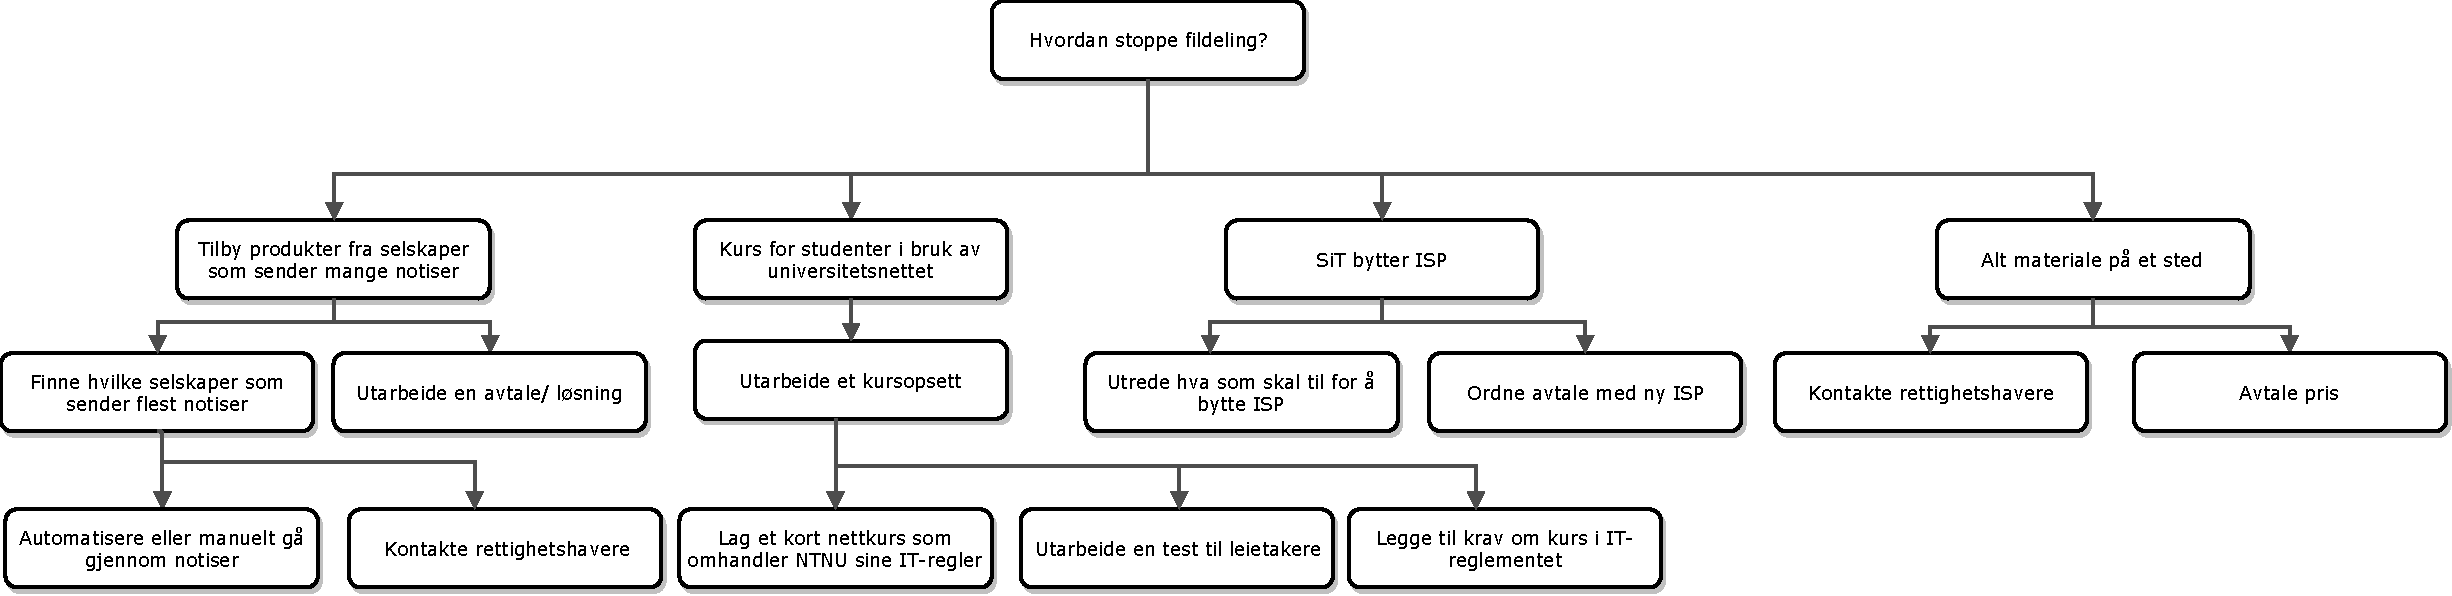
\includegraphics[scale=0.55, angle=90]{case_1/bilder/Tre-diagram.pdf}
    \caption[Trediagram til tiltak for case 1]{Løsningsimplementering}
    \label{fig:Tre-diagram}
\end{figure}

\subsection{Konklusjon av verktøy}
Dette verktøyet fungerte bra for å lage en plan til hvordan tiltakene skal bli implementert og hva som skal til for at tiltaket blir implementert. Trediagram er god måte å stykke opp arbeidsoppgavene for å skape en visuell prosess med oppgavene som må bli gjort for å nå målet.
\chapter{Diskusjon og konklusjon}


\bibliographystyle{ntnuthesis/ntnubachelorthesis}
\bibliography{case_1/bibliografi}

\appendix %after this line all chapters will have leters instead of numbers
%\input{projectplan}
%\input{gantt}
%\chapter{Meeting Logs}
You should include in the Appendix a log of your meeting.
\section{Temporal record of meetings}
\subsection*{11.01.2016 - Bachelor Information Meeting}
Discussion of the process and setup of the thesis.  Deadlines for submission of documentation.  Introduction to the process and the sessions to help with writing the thesis....

\subsection*{12.01.2016}
Met with supervisor to discuss the project. Actions:
\begin{enumerate}
	\item decide on a writing tool
	\item install development environment
	\item draft agreements by next week.
\end{enumerate}



%\input{progressreviews}
%\input{worklog}

\end{document}